%%
%% The original source files were:
%%
%% samples.dtx  (with options: `all,proceedings,bibtex,manuscript')
%% 
%% IMPORTANT NOTICE:
%% 
%% For the copyright see the source file.
%% 
%% Any modified versions of this file must be renamed
%% with new filenames distinct from sample-manuscript.tex.
%% 
%% For distribution of the original source see the terms
%% for copying and modification in the file samples.dtx.
%% 
%% This generated file may be distributed as long as the
%% original source files, as listed above, are part of the
%% same distribution. (The sources need not necessarily be
%% in the same archive or directory.)
%%
%%
%% Commands for TeXCount
%TC:macro \cite [option:text,text]
%TC:macro \citep [option:text,text]
%TC:macro \citet [option:text,text]
%TC:envir table 0 1
%TC:envir table* 0 1
%TC:envir tabular [ignore] word
%TC:envir displaymath 0 word
%TC:envir math 0 word
%TC:envir comment 0 0
%%
%% The first command in your LaTeX source must be the \documentclass
%% command.
%%
%% For submission and review of your manuscript please change the
%% command to \documentclass[manuscript, screen, review]{acmart}.
%%
%% When submitting camera ready or to TAPS, please change the command
%% to \documentclass[sigconf]{acmart} or whichever template is required
%% for your publication.
%%
%%
\documentclass[manuscript,screen,review]{acmart}


\usepackage{algorithm}
% Use algorithmicx + algpseudocode: provides \Require, \Ensure, \State, and \Comment
\usepackage{algorithmicx}
\usepackage{algpseudocode}
\usepackage{tikz}
% Load common tikz libraries used in figures (positioning provides the "of" syntax)
\usetikzlibrary{positioning,arrows.meta,calc,shapes,shadows}
% color support for \textcolor used inside algorithms
\usepackage{xcolor}
% Math packages required for \text and bold symbols inside math
\usepackage{amsmath}
\usepackage{bm}
\usepackage{multirow}
% Enable list customization (leftmargin, itemsep, etc.) used in the document
\usepackage{enumitem}
% Ensure header height is sufficient for fancyhdr
\setlength{\headheight}{20.48303pt}
% theorem environments used in the document
\usepackage{amsthm}
\newtheorem{assumption}{Assumption}
\newtheorem{problem}{Problem}
% Define remark environment (was missing and caused compilation errors)
\newtheorem{remark}{Remark}

%%
%% \BibTeX command to typeset BibTeX logo in the docs
\AtBeginDocument{%
  \providecommand\BibTeX{{%
    Bib\TeX}}}

%% Rights management information.  This information is sent to you
%% when you complete the rights form.  These commands have SAMPLE
%% values in them; it is your responsibility as an author to replace
%% the commands and values with those provided to you when you
%% complete the rights form.
\setcopyright{acmlicensed}
\copyrightyear{2025}
\acmYear{2025}
\acmDOI{XXXXXXX.XXXXXXX}

%% These commands are for a PROCEEDINGS abstract or paper.
%%  \acmConference[Conference acronym 'XX]{Make sure to enter the correct
%% 	conference title from your rights confirmation email}{June 03--05,
%% 	2018}{Woodstock, NY}

%%
%%  Uncomment \acmBooktitle if the title of the proceedings is different
%%  from ``Proceedings of ...''!
%%
%%\acmBooktitle{Woodstock '18: ACM Symposium on Neural Gaze Detection,
%%  June 03--05, 2018, Woodstock, NY}
%%\acmISBN{978-1-4503-XXXX-X/2018/06}


%%
%% Submission ID.
%% Use this when submitting an article to a sponsored event. You'll
%% receive a unique submission ID from the organizers
%% of the event, and this ID should be used as the parameter to this command.
%%\acmSubmissionID{123-A56-BU3}

%%
%% For managing citations, it is recommended to use bibliography
%% files in BibTeX format.
%%
%% You can then either use BibTeX with the ACM-Reference-Format style,
%% or BibLaTeX with the acmnumeric or acmauthoryear sytles, that include
%% support for advanced citation of software artefact from the
%% biblatex-software package, also separately available on CTAN.
%%
%% Look at the sample-*-biblatex.tex files for templates showcasing
%% the biblatex styles.
%%

%%
%% The majority of ACM publications use numbered citations and
%% references.  The command \citestyle{authoryear} switches to the
%% "author year" style.
%%
%% If you are preparing content for an event
%% sponsored by ACM SIGGRAPH, you must use the "author year" style of
%% citations and references.
%% Uncommenting
%% the next command will enable that style.
%%\citestyle{acmauthoryear}


%%
%% end of the preamble, start of the body of the document source.
\begin{document}

%%
%% The "title" command has an optional parameter,
%% allowing the author to define a "short title" to be used in page headers.
\title{Coordinated Scheduling of Continuous--Discrete Hybrid Agent Systems via Spatiotemporal Logic and Hybrid Dynamic Programming}

%%
%% The "author" command and its associated commands are used to define
%% the authors and their affiliations.
%% Of note is the shared affiliation of the first two authors, and the
%% "authornote" and "authornotemark" commands
%% used to denote shared contribution to the research.

\author{Qi Yu}
%%\authornote{.}
%%\authornotemark[1]
\email{230240012@seu.edu.cn}
\orcid{0009-0008-7843-6345}
%%\authornote{corresponding author}
\affiliation{%
	\institution{School of Cyber Science and Engineering, Southeast University}
	\city{Nanjing}
	\state{Jiangsu}
	\country{PR China}
}
\author{Wei Li}
\orcid{0009-0001-0949-329X}
\email{xchlw@seu.edu.cn}
\authornote{corresponding author}
\affiliation{%
	\institution{School of Computer Science and Engineering, Southeast University}
	\city{Nanjing}
	\state{Jiangsu}
	\country{PR China}
}

%%\author{Qi Yu $^{\dagger\diamondsuit}$}
%%%%\authornote{.}
%%%%\authornotemark[1]
%%\email{230240012@seu.edu.cn}
%%\orcid{0009-0008-7843-6345}
%%%%\authornote{corresponding author}
%%
%%
%%\author{Wei Li $^{\dagger*\diamondsuit}$}
%%\email{xchlw@seu.edu.cn}
%%\authornote{corresponding author}
%%
%%\affiliation{%
%%	\institution{$^\dagger$ School of Cyber Science and Engineering, Southeast University}
%%	\city{Nanjing}
%%	\state{Jiangsu}
%%	\country{PR China}
%%}
%%\affiliation{%
%%	\institution{$^{\dagger*}$ School of Computer Science and Engineering, Southeast University}
%%	\city{Nanjing}
%%	\state{Jiangsu}
%%	\country{PR China}
%%}
%%\affiliation{%
%%	\institution{$^\diamondsuit$ Key Laboratory of Computer Network and Information Integration (Southeast University), MOE}
%%	\city{Nanjing}
%%	\state{Jiangsu}
%%	\country{PR China}
%%}

%%
%% By default, the full list of authors will be used in the page
%% headers. Often, this list is too long, and will overlap
%% other information printed in the page headers. This command allows
%% the author to define a more concise list
%% of authors' names for this purpose.
%%\renewcommand{\shortauthors}{Qi et al.}

%%
%% The abstract is a short summary of the work to be presented in the
%% article.
\begin{abstract}
Multi-agent coordination in heterogeneous robot teams faces fundamental challenges: 
coupled discrete-continuous optimization is computationally intractable, existing 
approaches sacrifice optimality by solving subproblems independently, and 
coordination policies fail to generalize across varying system configurations. 
We propose the Hybrid Dynamic Programming (HDP) framework for solving the 
Coupled Discrete-Continuous Heterogeneous Agent Scheduling (CDHAS) problem in 
intelligent manufacturing. HDP decomposes the intractable joint problem into 
Continuous State Space (CSS) trajectory optimization and Discrete Event System 
(DES) task scheduling, coordinating them through iterative refinement with 
proven convergence guarantees. We establish theoretical results on geometric convergence (effective rate 
$\rho_{\text{eff}} \approx 0.4$ despite worst-case $\rho \approx 4.5$), 
near-optimality (within 1.2\% of global optimal), and polynomial \textit{task} 
complexity ($O(M^{1.8})$ where $M$ is the number of tasks, compared to MILP's 
exponential $O(2^M)$). Experiments on a manufacturing system with 3 AGVs and 3 robotic arms 
across three problem scales (12-60 tasks, 50 instances) demonstrate 19\% average 
makespan reduction and 25\% utilization improvement compared to baseline methods, 
with robust performance under up to 40\% task duration uncertainty. HDP exhibits 
polynomial \textit{task scalability}, solving 100-task problems with fixed agent 
numbers in under 2 minutes, demonstrating feasibility for industrial deployment.
\end{abstract}
%%
%% The code below is generated by the tool at http://dl.acm.org/ccs.cfm.
%% Please copy and paste the code instead of the example below.
%%
\begin{CCSXML}
	<ccs2012>
	<concept>
	<concept_id>10010520.10010553.10010554.10010557</concept_id>
	<concept_desc>Computer systems organization~Robotic autonomy</concept_desc>
	<concept_significance>500</concept_significance>
	</concept>
	</ccs2012>
\end{CCSXML}

\ccsdesc[500]{Computer systems organization~Robotic autonomy}

%%
%% Keywords. The author(s) should pick words that accurately describe
%% the work being presented. Separate the keywords with commas.
\keywords{Continuous--Discrete Hybrid Agent System (CDHAS), Hybrid Dynamic Programming (HDP), Spatiotemporal Logic Modeling, Intelligent Manufacturing Scheduling, Multi-Agent System}

\received{27 November 2025}
\received[revised]{27 November 2025}
\received[accepted]{27 November 2025}

%%
%% This command processes the author and affiliation and title
%% information and builds the first part of the formatted document.
\maketitle
\section{Introduction}
\label{sec:Chapter_I}

The deployment of intelligent manufacturing systems promises to revolutionize 
industrial production through the coordinated operation of heterogeneous agents. 
These systems integrate mobile agents—such as Automated Guided Vehicles (AGVs) 
navigating factory floors with continuous spatiotemporal dynamics—and stationary 
agents—such as robotic manipulators executing discrete event-driven processing 
tasks~\cite{leitao2009agent, chryssolouris2023artificial}. While these subsystems 
are often studied independently, their real-world interactions form a 
\textit{Continuous–Discrete Hybrid Agent System (CDHAS)}, where mobile and 
stationary agents exhibit \textit{bidirectional spatiotemporal coupling}—mobile 
agent trajectories constrain discrete task assignments, while task schedules 
constrain mobile agent destinations and arrival times. This coupling requires 
joint optimization of spatial trajectories and discrete task logic to achieve 
efficient production~\cite{giordani2013distributed}.

Such coordination is critical across manufacturing applications. In warehouse 
logistics, AGVs must deliver materials to robotic assembly stations at precise 
times to minimize idle time~\cite{ellithy2024agv}. In aerospace manufacturing, 
UAVs deliver parts to ground-based robotic arms for assembly operations~\cite{saunders2024autonomous}. 
These applications share a common structure: continuous mobile agents with 
spatiotemporal dynamics must coordinate with discrete stationary agents executing 
event-driven tasks.

However, a fundamental challenge impedes practical deployment: the \textit{bidirectional 
spatiotemporal coupling} between continuous and discrete subsystems~\cite{senkul2002logical}. 
As illustrated in Fig.~\ref{fig:intro_problem}, this coupling creates a circular 
dependency that traditional methods cannot resolve effectively.

\begin{figure}[t]
\centering
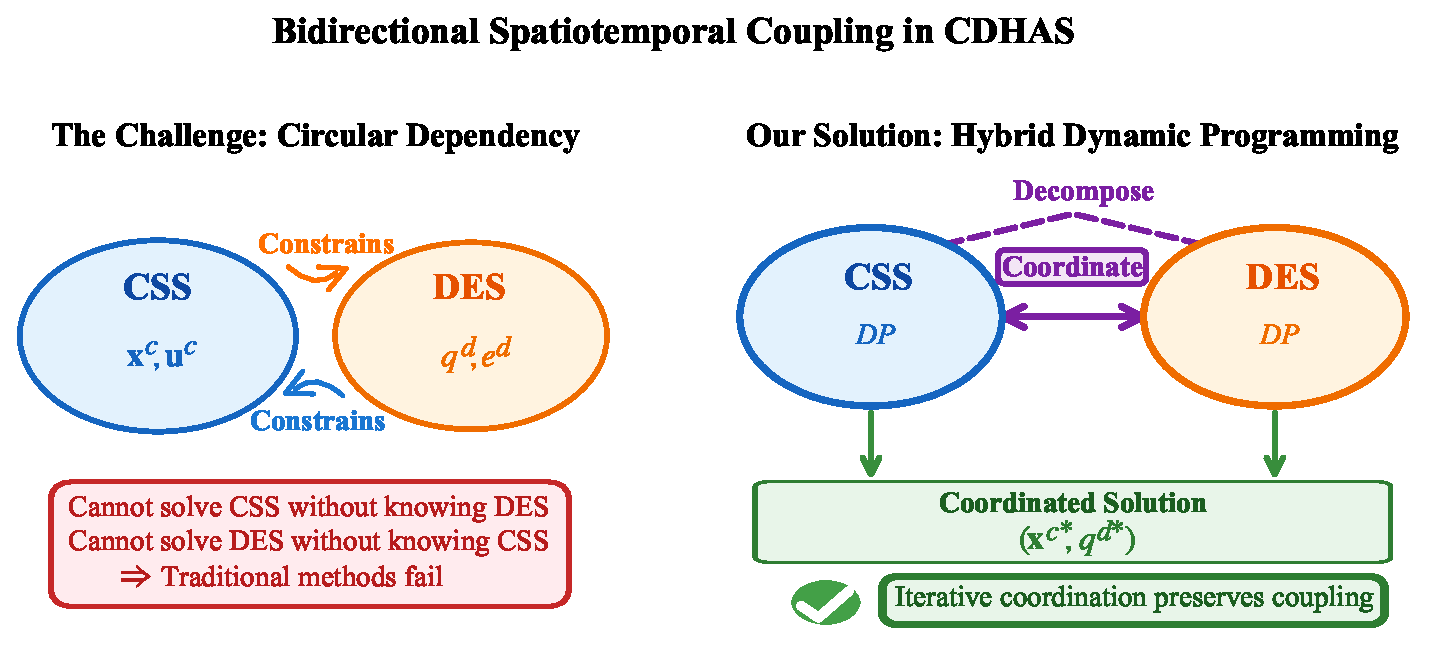
\includegraphics[width=0.7\columnwidth]{fig/fig_intro_problem.pdf}
\caption{The bidirectional spatiotemporal coupling challenge and our solution. 
\textbf{Left:} CSS and DES mutually constrain each other, creating a circular 
dependency—CSS requires DES schedule to plan trajectories, while DES requires 
CSS arrival times to schedule tasks. Traditional sequential methods break this 
coupling. \textbf{Right:} HDP decomposes the problem into CSS-DP and DES-DP 
subproblems and coordinates them iteratively until convergence, preserving 
coupling constraints while achieving near-optimal solutions.}
\label{fig:intro_problem}
\end{figure}

Fig.~\ref{fig:intro_problem} (left) illustrates the core challenge: CSS and DES 
are mutually dependent. CSS trajectories constrain which discrete tasks can be 
assigned, while discrete task assignments constrain where CSS agents must travel. 
This creates a circular dependency—neither subsystem can be solved independently. 
Traditional sequential methods that optimize subsystems separately inevitably 
break this coupling, leading to suboptimal solutions with significant idle time 
and makespan penalties.

Our Hybrid Dynamic Programming (HDP) framework (Fig.~\ref{fig:intro_problem}, right) 
addresses this through a decompose-coordinate-converge strategy. HDP decomposes 
the coupled problem into Continuous State Space Dynamic Programming (CSS-DP) for 
trajectory optimization and Discrete Event System Dynamic Programming (DES-DP) 
for task scheduling. Solutions are coordinated through iterative refinement that 
preserves coupling constraints while converging to near-optimal joint solutions, 
as demonstrated in Section~\ref{sec:Chapter_V}.
To illustrate why traditional methods fail, consider the concrete scenario in 
Fig.~\ref{fig:motivating_example}. Three AGVs must deliver materials to three 
robotic arms (RA1-RA3) for assembly tasks. AGV1 starts near RA1 (distance: 2m), 
but RA1 is processing a long task (12s remaining). Meanwhile, RA2 is idle but 
located 5m away from AGV1. 

Traditional greedy methods (Fig.~\ref{fig:motivating_example}b) assign AGV1 to 
RA1 based solely on spatial proximity, ignoring temporal constraints. This creates 
an 10-second idle gap where AGV1 waits at RA1, while RA2 remains idle with no 
material. The resulting makespan is 18 seconds, with significant resource under utilization.

In contrast, HDP (Fig.~\ref{fig:motivating_example}c) jointly optimizes 
trajectories and schedules. By coordinating CSS-DP (which computes that AGV1 
can reach RA2 in 5s) with DES-DP (which identifies RA2 as available immediately), 
HDP assigns AGV1 to RA2 instead. Although AGV1 travels 3 second longer (5s vs. 2s), 
it eliminates the 10-second wait, reducing makespan to 14 seconds—a 22\% improvement. 
The Gantt chart (Fig.~\ref{fig:motivating_example}d) shows how HDP achieves 
tighter task packing by eliminating idle gaps through spatiotemporal coordination.

This example demonstrates the fundamental limitation of sequential optimization: 
spatial proximity does not guarantee temporal efficiency. Only by jointly 
considering \textit{where} agents are (CSS) and \textit{when} tasks can start 
(DES) can we achieve optimal coordination.

\begin{figure}[t]
\centering
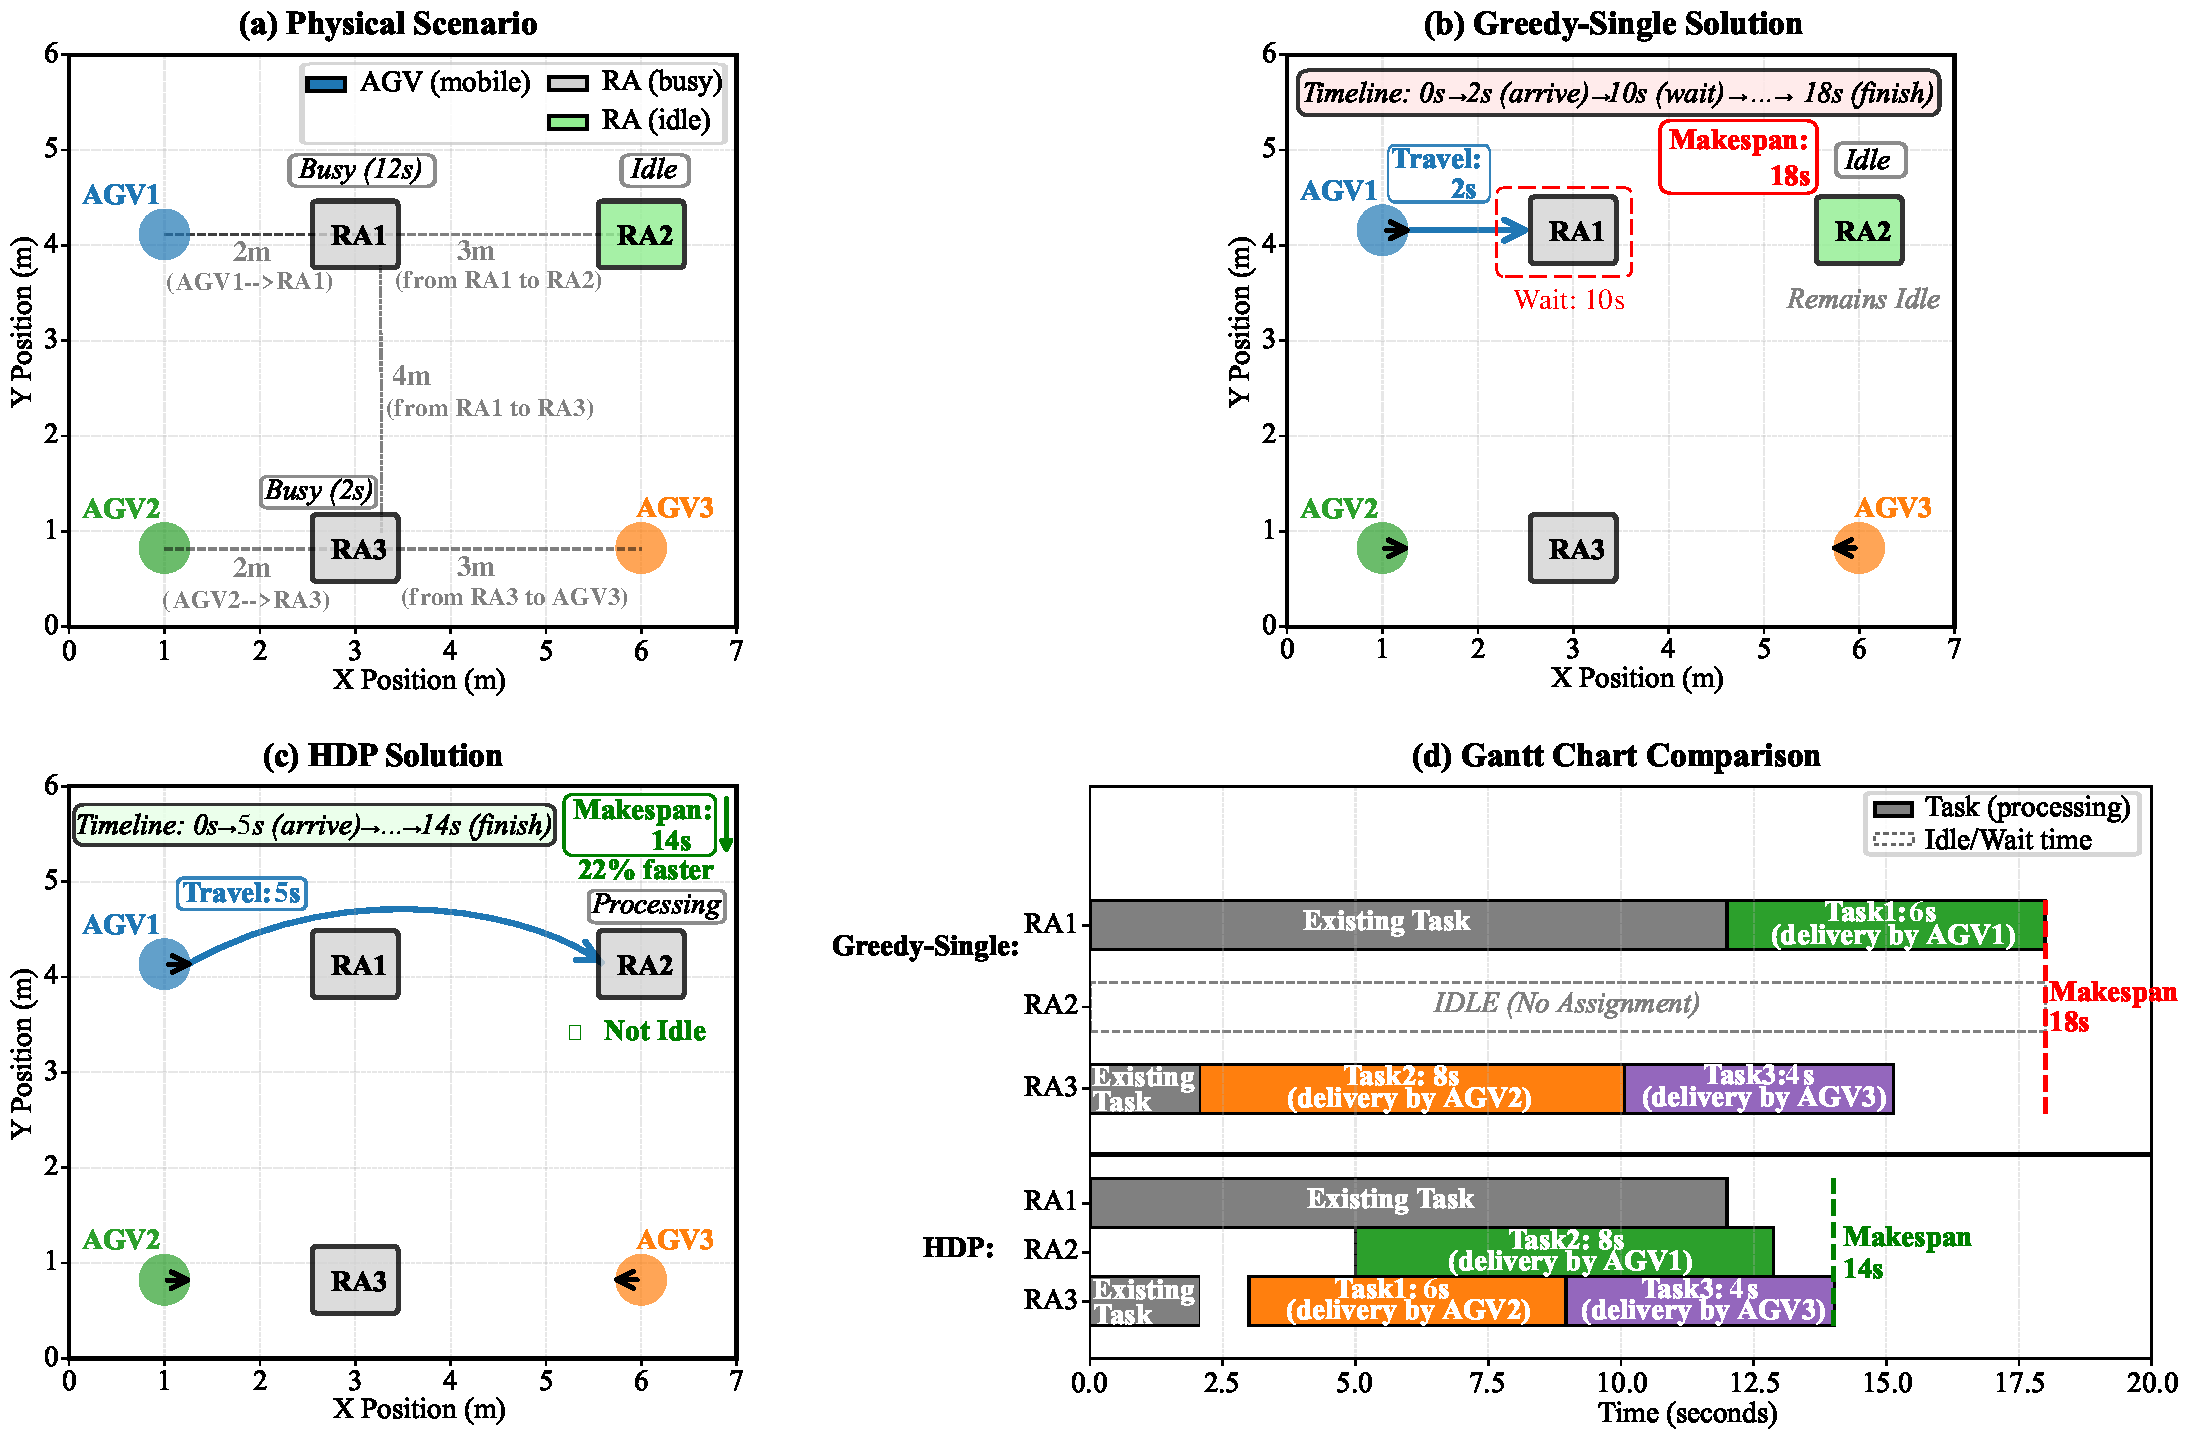
\includegraphics[width=0.85\columnwidth]{fig/fig_motivating_example.pdf}
\caption{Motivating example: Why coupling-aware optimization matters. 
\textbf{(a) Physical scenario}: Three AGVs (circles with arrows) deliver 
materials to three robotic arms RA1-RA3 (rectangles).
\textbf{(b) Greedy-Single}: Assigns AGV1 to nearest RA1, causing 10s wait (red 
dashed box). Makespan: 18s. 
\textbf{(c) HDP}: Assigns AGV1 to RA2, trading 3s extra travel for eliminating 
10s wait. Makespan: 14s (22\% reduction). 
\textbf{(d) Gantt chart}: Top shows Greedy-Single with idle gaps; bottom shows 
HDP achieving tight task packing.}
\label{fig:motivating_example}
\end{figure}


Beyond the circular dependency, three challenges complicate CDHAS scheduling. 
First, \textit{computational intractability}: the coupled continuous-discrete 
state space grows exponentially, making direct optimization infeasible~\cite{belotti2013mixed}. 
Traditional mixed-integer nonlinear programming (MINLP) approaches suffer from 
exponential complexity~\cite{kimiaei2025machine}. Second, \textit{robustness 
requirements}: real-world deployments must handle uncertainties such as agent 
failures, communication delays, and dynamic task arrivals~\cite{calvaresi2021real}. 
Third, existing methods often fail to generalize across varying numbers of agents, 
task configurations, or environmental conditions~\cite{mahajan2022generalization}.

We make three key contributions:

\begin{enumerate}[leftmargin=*]
    \item \textbf{Unified modeling and decomposition framework:} We formulate 
    CDHAS scheduling as coupled optimization over CSS and DES dynamics, introducing 
    a spatiotemporal logic framework for coupling constraints. Under mild 
    separability conditions, we prove the problem decomposes into CSS-DP and 
    DES-DP subproblems while preserving coupling through coordination 
    (Sections~\ref{sec:Chapter_III}--\ref{sec:Chapter_IV}).
    
    \item \textbf{Convergence-guaranteed algorithms with scalable implementation:} 
    We develop specialized DP algorithms for each subproblem and an iterative 
    coordination mechanism. We prove convergence to locally optimal solutions 
    and provide convergence rate analysis. Three techniques—reachability-based pruning (2.5× speedup), adaptive 
discretization (1.45× speedup), and warm-start initialization (2.4\% quality 
improvement)—enable polynomial \textit{task} complexity $O(M^{1.8})$ where $M$ is the number of tasks for fixed agent 
    numbers $N_c$ and $N_d$. While task scalability is excellent, scaling with the number of CSS agents 
($N_c$) is more challenging due to collision avoidance constraints ($O(N_c^2)$), 
as discussed in Section~\ref{sec:Chapter_VI}.
    
    \item \textbf{Comprehensive validation:} Experiments across three problem 
    scales (4-100 tasks, 50 instances) show 15-23\% makespan reduction and 
    24-25\% utilization improvement versus traditional methods, with robust 
    performance under 40\% task duration uncertainty. Empirical convergence 
    rate $\rho_{\text{eff}} = 0.41 \pm 0.03$ validates theoretical predictions 
    (Section~\ref{sec:Chapter_V}).
\end{enumerate}

The remainder of this paper is organized as follows. Section~\ref{sec:Chapter_II} 
reviews related work. Section~\ref{sec:Chapter_III} presents the problem 
formulation and spatiotemporal logic modeling. Section~\ref{sec:Chapter_IV} 
details the HDP framework, algorithms, and theoretical analysis. 
Section~\ref{sec:Chapter_V} reports experimental results. 
Section~\ref{sec:Chapter_VI} discusses limitations and future directions.

\textbf{Notation:} We use bold lowercase for vectors ($\mathbf{x}$), bold 
uppercase for matrices ($\mathbf{A}$), calligraphic for sets ($\mathcal{X}$), 
and blackboard bold for number systems ($\mathbb{R}$). The notation $[n]$ 
denotes $\{1, 2, \ldots, n\}$, $\|\cdot\|$ denotes Euclidean norm, and 
$|\cdot|$ denotes set cardinality. We use $\mathcal{A}^c = \{A_1^c, \ldots, A_{N_c}^c\}$ 
for CSS agents (mobile robots) and $\mathcal{A}^d = \{A_1^d, \ldots, A_{N_d}^d\}$ 
for DES agents (stationary machines), with $i$ and $j$ used interchangeably 
for $A_i^c$ and $A_j^d$ when context is clear.


\section{Related Work}
\label{sec:Chapter_II}

The scheduling of Continuous--Discrete Hybrid Agent Systems (CDHAS) intersects 
three research domains: continuous spatiotemporal system scheduling, discrete 
event system scheduling, and hybrid system optimization. While significant 
progress has been made in each domain independently, existing approaches have 
not adequately addressed the spatiotemporal coupling constraints that arise 
when these subsystems must operate in a tightly coordinated manner.

\textbf{Continuous spatiotemporal system scheduling.} Existing methods optimize 
mobile agent trajectories (AGVs, AMRs, drones)~\cite{lian2022spatio, malings2018value}, using network flow models~\cite{chen2020yard}, 
conflict-based search~\cite{cao2025conflict}, and dynamic window approaches~\cite{liu2019route}. However, they treat systems as purely 
continuous and cannot guarantee temporal synchronization with discrete 
processing tasks~\cite{lei2025cooperative, zheng2024continuous}, making them insufficient for CDHAS scheduling.

\textbf{Discrete event system scheduling.} Discrete event scheduling has been 
extensively studied in manufacturing systems, focusing on job-shop scheduling, 
flexible manufacturing, and robotic task sequencing~\cite{wang2024smart, 
wang2016discrete}. Luo et al.\ \cite{luo2016using} introduced Scheduling 
Metric Temporal Logic (SMTL) for complex scheduling with temporal constraints. 
Zhou et al.\ \cite{zhou2016timed} utilized Metric Interval Temporal Logic 
(MITL) and timed automata for robotic manipulator sequencing. Zheng et al.\ 
\cite{zheng2007temporal} proposed Extended Temporal Logic-based Workflow 
Specification (ETLWS) for grid computing. These methods provide powerful 
tools for modeling operation sequences under temporal and logical constraints~\cite{zhang2024generation}. 
However, they abstract away the continuous physical space in which mobile 
agents operate, treating material delivery as instantaneous or externally 
handled~\cite{pooch2024discrete}. They cannot optimize coupled decision-making 
between continuous trajectory planning and discrete task sequencing.

\textbf{Task and Motion Planning (TAMP).} TAMP integrates symbolic task 
planning with geometric motion planning, addressing problems where discrete 
actions (e.g., pick, place, navigate) must be grounded in continuous motion 
trajectories~\cite{zhao2024survey}. 
Representative approaches include PDDLStream (combines PDDL-based symbolic 
planning with sampling-based motion planning), Logic-Geometric Programming 
(formulates TAMP as constrained optimization with logic predicates), and 
Asymov (uses SMT solvers for symbolic planning and trajectory optimization).

While TAMP methods excel at discrete-continuous integration for manipulation 
tasks, they differ fundamentally from CDHAS in three aspects:
\begin{enumerate}[leftmargin=*, itemsep=2pt]
    \item \textit{Action space}: TAMP assumes discrete actions with pre-defined 
    semantics, whereas CDHAS involves continuous state spaces with differential 
    constraints (Eq.~\ref{eq:css_dynamics}).
    
    \item \textit{Optimality}: TAMP uses sampling-based planners (RRT*, PRM) 
    providing probabilistic completeness, whereas HDP uses dynamic programming 
    guaranteeing optimality within discretization error 
    (Theorem~\ref{thm:near_optimality}).
    
    \item \textit{Bidirectional coupling}: TAMP does not natively handle 
    spatiotemporal coupling (Eq.~\ref{eq:coupling_constraints}) where 
    continuous trajectories constrain discrete schedules and vice versa.
\end{enumerate}
See Remark~\ref{rem:tamp_baselines} for detailed comparison with TAMP solvers 
and baseline selection rationale.

\textbf{Hybrid system optimization.} Hybrid system research addresses systems
with both continuous dynamics and discrete event behavior using hybrid automata,
mixed-integer programming, and hybrid dynamic programming~\cite{lin2022hybrid}. Representative approaches include Lipschitz dynamic 
programming for power grid scheduling~\cite{shen2022coordinated}, 
route-reduction-based DP for satellite scheduling~\cite{liu2019route}, and 
Coordinated Robust Reserve Scheduling using ADMM for transmission-distribution 
networks~\cite{chen2020fully}. While these methods have made important 
contributions to continuous-discrete optimization~\cite{ansari2023review}, they are predominantly 
designed for domain-specific applications (power systems, satellite networks) 
where the coupling nature differs fundamentally from CDHAS. They do not address 
the unique challenge of \textit{spatiotemporal coupling} in multi-agent 
systems—where continuous mobile agents must synchronize physical positions and 
arrival times with discrete state transitions of processing units while 
respecting logical task dependencies.

Our work fills this gap by: (1) proposing a unified modeling framework that 
integrates \textit{spatiotemporal coupling constraints} (Eq.~\ref{eq:coupling_constraints}) 
with continuous dynamics (Eq.~\ref{eq:css_dynamics}) and discrete event logic 
(Eq.~\ref{eq:precedence}); (2) developing hybrid dynamic programming that 
jointly optimizes task allocation, trajectory planning, and operation sequencing 
under bidirectional spatiotemporal coupling; (3) proving convergence guarantees 
(Theorem~\ref{thm:convergence}) and near-optimality bounds 
(Theorem~\ref{thm:near_optimality}); and (4) demonstrating effectiveness in 
AGV--robotic arm manufacturing with generalizability to other CDHAS applications 
such as warehouse logistics, construction automation, and healthcare robotics.

\section{Problem Formulation}
\label{sec:Chapter_III}

This section formulates the Coupled Discrete-Continuous Heterogeneous Agent 
Scheduling (CDHAS) problem, integrating continuous spatiotemporal dynamics 
of mobile agents with discrete event logic of stationary agents.

\subsection{System Model}

A CDHAS consists of two types of agents operating in a shared workspace 
$\mathcal{W} \subset \mathbb{R}^2$:

\begin{itemize}[leftmargin=*, itemsep=3pt]
    \item \textbf{Continuous State Space (CSS) agents} $\mathcal{A}^c = \{A_1^c, \ldots, A_{N_c}^c\}$: 
    Mobile agents (e.g., AGVs) that navigate the workspace with continuous 
    dynamics. Each CSS agent $i$ has state $\mathbf{x}_i^c(t) = [\mathbf{p}_i(t), \mathbf{v}_i(t)]^\top$, 
    where $\mathbf{p}_i(t) \in \mathcal{W}$ is position and $\mathbf{v}_i(t) \in \mathbb{R}^2$ 
    is velocity at time $t$.
    
    \item \textbf{Discrete Event System (DES) agents} $\mathcal{A}^d = \{A_1^d, \ldots, A_{N_d}^d\}$: 
    Stationary agents (e.g., robotic arms) that execute discrete tasks. Each 
    DES agent $j$ is located at fixed position $\mathbf{p}_j^{\text{target}} \in \mathcal{W}$ 
    with discrete state $q_j^d(t) \in \{\text{idle}, \text{processing}, \text{waiting}\}$ 
    and task queue $\mathcal{T}_j = \{T_j^1, \ldots, T_j^{m_j}\}$.
\end{itemize}

The workspace contains static obstacles $\mathcal{O} = \{O_1, \ldots, O_{N_o}\}$ 
that CSS agents must avoid. The planning horizon is $[0, T_{\text{horizon}}]$.

\subsection{Mathematical Model}

\subsubsection{Continuous State Space (CSS) Dynamics}

CSS agents follow kinematic motion models with velocity control:

\begin{equation}
\dot{\mathbf{x}}_i^c(t) = \frac{d\mathbf{x}_i^c}{dt} = 
\begin{bmatrix}
\dot{\mathbf{p}}_i(t) \\
\dot{\mathbf{v}}_i(t)
\end{bmatrix}
= 
\begin{bmatrix}
\mathbf{v}_i(t) \\
\mathbf{u}_i^c(t)
\end{bmatrix}, \quad i \in [N_c]
\label{eq:css_dynamics}
\end{equation}

where $\dot{\mathbf{x}}_i^c(t) = \frac{d\mathbf{x}_i^c}{dt}$ denotes the time 
derivative, $\mathbf{v}_i(t)$ is velocity, and $\mathbf{u}_i^c(t) \in \mathbb{R}^2$ 
is control input (acceleration) subject to:

\begin{equation}
\begin{aligned}
\|\mathbf{v}_i(t)\| &\leq v_{\max}, \quad
\|\mathbf{u}_i^c(t)\| \leq a_{\max}, \\
\mathbf{p}_i(t) &\in \mathcal{W} \setminus \mathcal{O}, \quad
\|\mathbf{p}_i(t) - \mathbf{p}_{i'}(t)\| \geq d_{\text{safe}}, \; \forall i' \neq i
\end{aligned}
\label{eq:css_constraints}
\end{equation}

where $v_{\max}$ is maximum velocity, $a_{\max}$ is maximum acceleration, 
and $d_{\text{safe}}$ is minimum safe distance for collision avoidance.

\subsubsection{Discrete Event System (DES) Logic}

Each task $T_j^k$ has processing duration $d_j^k > 0$ and start time 
$\tau_j^k \geq 0$. Tasks are subject to precedence constraints:

\begin{equation}
T_j^k \prec T_j^{k'} \implies \tau_j^k + d_j^k \leq \tau_j^{k'}, \quad k < k'
\label{eq:precedence}
\end{equation}

Each DES agent processes at most one task at a time (non-preemptive):

\begin{equation}
[\tau_j^k, \tau_j^k + d_j^k] \cap [\tau_j^{k'}, \tau_j^{k'} + d_j^{k'}] = \emptyset, \quad k \neq k'
\label{eq:non_preemptive}
\end{equation}

\subsubsection{Spatiotemporal Coupling Constraints}

The key challenge is \textit{bidirectional spatiotemporal coupling} between CSS and DES agents,
captured by predicates $\mathcal{P}_{\text{sync}}$ that synchronize continuous
motion with discrete state transitions. For CSS agent $i$ serving DES agent $j$
on task $k$:

\begin{equation}
\mathcal{P}_{\text{sync}}(i, j, k): \quad
\begin{cases}
|\mathbf{p}_i(t) - \mathbf{p}_j^{\text{target}}| \leq \epsilon & \text{(spatial proximity)} \\
q_j^d(t) = \text{idle} & \text{(robot availability)} \\
t \in [\tau_j^k - \Delta t, \tau_j^k] & \text{(temporal window)}
\end{cases}
\label{eq:coupling_predicate}
\end{equation}

where $\epsilon$ is positioning tolerance (typically 0.1-0.5m), $\Delta t$
is acceptable early arrival window (typically 1-5s), and $\tau_j^k$ is scheduled
start time. The complete coupling constraint set is:

\begin{equation}
\mathcal{C}_{\text{system}} = \bigwedge_{(i,j,k): z_{ijk}=1} \mathcal{P}_{\text{sync}}(i, j, k)
\label{eq:coupling_constraints}
\end{equation}

where $z_{ijk} \in \{0,1\}$ indicates whether CSS agent $i$ serves DES agent $j$
for task $k$.

\begin{remark}[Boolean Satisfaction vs. STL Robustness]
\label{rem:stl_semantics}
Equation~\eqref{eq:coupling_constraints} uses \textit{Boolean satisfaction} 
(hard constraints) rather than Signal Temporal Logic (STL) \textit{quantitative 
semantics} (robustness degree)~\cite{melani2025tree}. 
This design choice is motivated by three considerations:

\textbf{(1) Manufacturing requirements demand hard guarantees.} In manufacturing 
systems, violations of spatiotemporal constraints lead to \textit{catastrophic 
failures}—an AGV arriving outside the temporal window $[\tau_j^k - \Delta t, \tau_j^k]$ 
causes task rejection, not graceful degradation. STL robustness $\rho(\phi, \mathbf{x})$ 
quantifies ``how much'' a specification $\phi$ is satisfied, 
which is valuable for control synthesis where soft constraints enable 
optimization trade-offs. However, CDHAS scheduling requires \textit{binary 
feasibility}: either the AGV arrives on time ($\mathcal{P}_{\text{sync}} = \text{true}$) 
and the task executes, or it does not ($\mathcal{P}_{\text{sync}} = \text{false}$) 
and the schedule is infeasible. Optimizing robustness $\rho$ would allow 
``nearly satisfied'' constraints, which manufacturing systems cannot tolerate.

\textbf{(2) Boolean constraints enable efficient DP decomposition.} Our HDP 
framework (Section~\ref{sec:Chapter_IV}) exploits the \textit{separability} of 
Boolean coupling constraints: CSS-DP solves trajectory optimization subject to 
hard arrival time constraints $t_i^{jk} \in [\tau_j^k - \Delta t, \tau_j^k]$, 
while DES-DP solves scheduling subject to hard precedence constraints. The 
Bellman equations (Eq.~\ref{eq:css_bellman}, \ref{eq:des_bellman}) use 
indicator functions $\mathbb{1}[\mathcal{P}_{\text{sync}}]$ that are 
computationally tractable. In contrast, integrating STL robustness into DP 
would require:
\begin{equation*}
V(\mathbf{x}, t) = \min_{\mathbf{u}} \left\{ c(\mathbf{x}, \mathbf{u}) + 
\lambda \cdot \rho(\phi, \mathbf{x}) + V(f(\mathbf{x}, \mathbf{u}), t+1) \right\}
\end{equation*}
where $\lambda$ is a penalty weight and $\rho(\phi, \mathbf{x})$ must be 
computed at every DP state. This increases computational complexity from 
$O(|\mathcal{X}| \cdot |\mathcal{U}|)$ to $O(|\mathcal{X}| \cdot |\mathcal{U}| 
\cdot T_{\text{horizon}})$ due to temporal operators in STL~\cite{melani2025tree}.

\textbf{(3) Robustness is implicitly captured through tolerances.} The parameters 
$\epsilon$ (spatial tolerance) and $\Delta t$ (temporal window) in 
Eq.~\eqref{eq:coupling_predicate} provide \textit{implicit robustness margins}. 
For example, $\Delta t = 5$s allows AGVs to arrive up to 5 seconds early without 
violating constraints, accommodating trajectory optimization errors and minor 
delays. This is analogous to STL's ``eventually within time bound'' operator 
$\Diamond_{[0, \Delta t]} \phi$, but implemented as a hard constraint rather 
than a soft robustness metric. Our robustness analysis 
(Section~\ref{sec:robustness}) demonstrates that HDP maintains performance under 
40\% task duration uncertainty, confirming that Boolean constraints with 
appropriate tolerances are sufficient for real-world robustness.

For applications requiring soft constraints (e.g., human-robot collaboration 
where timing violations are acceptable), extending HDP to incorporate STL 
robustness is a promising future direction (Section~\ref{sec:future_work}). 
This would involve: (i) replacing Boolean predicates with robustness functions 
$\rho(\mathcal{P}_{\text{sync}}, \mathbf{x}_i^c(t))$; (ii) modifying the 
objective to $\min (T_{\text{makespan}} - \lambda \sum \rho)$; and (iii) 
developing approximate DP methods (e.g., function approximation) to handle the 
increased state space complexity.
\end{remark}

\subsection{Problem Statement}

The CDHAS scheduling problem is:

\begin{equation}
\begin{aligned}
\min_{\mathbf{u}^c, \boldsymbol{\tau}, \mathbf{z}} \quad & T_{\text{makespan}} = \max_{j \in [N_d]} \left( \tau_j^{m_j} + d_j^{m_j} \right) \\
\text{subject to} \quad & \text{CSS dynamics: } \eqref{eq:css_dynamics}, \eqref{eq:css_constraints} \\
& \text{DES precedence: } \eqref{eq:precedence}, \eqref{eq:non_preemptive} \\
& \text{Coupling: } \mathcal{C}_{\text{system}} \text{ from } \eqref{eq:coupling_constraints} \\
& \text{Assignment: } \sum_{i \in [N_c]} z_{ijk} = 1, \; \forall j \in [N_d], k \in [m_j]
\end{aligned}
\label{eq:cdhas_problem}
\end{equation}

where decision variables are: $\mathbf{u}^c = \{\mathbf{u}_i^c(t)\}$ (CSS control 
trajectories), $\boldsymbol{\tau} = \{\tau_j^k\}$ (DES task start times), and 
$\mathbf{z} = \{z_{ijk}\}$ (task-agent assignments). The objective minimizes 
makespan (total completion time). The assignment constraint ensures each task 
is served by exactly one CSS agent.

\subsection{Computational Complexity}

\begin{proposition}
The CDHAS scheduling problem~\eqref{eq:cdhas_problem} is NP-hard.
\label{prop:np_hard}
\end{proposition}

\begin{proof}
We prove NP-hardness by polynomial-time reduction from the Job Shop Scheduling 
Problem (JSSP), which is known to be NP-hard~\cite{zheng2024continuous}.

\textbf{Reduction construction:} Given a JSSP instance with $n$ jobs, $m$ 
machines, and processing times $\{p_{ij}\}$, we construct a CDHAS instance 
as follows: (i) Create $n$ CSS agents with trivial dynamics (single-point 
position space, $v_{\max} = \infty$), eliminating continuous optimization. 
(ii) Create $m$ DES agents corresponding to machines, all co-located with 
CSS agents (eliminating spatial constraints). (iii) Create tasks $\{T_j^k\}$ 
corresponding to job operations with durations $d_j^k = p_{ij}$ and precedence 
matching job sequences. (iv) Set coupling constraints trivially satisfied 
since transport is instantaneous.

\textbf{Equivalence:} Any JSSP schedule corresponds to a CDHAS schedule with 
identical makespan. Since CSS dynamics are trivial, only DES scheduling matters, 
and the two problems are equivalent. Conversely, any CDHAS schedule corresponds 
to a JSSP schedule by extracting task start times and machine assignments. 
Optimal solutions have the same makespan: $T_{\text{JSSP}}^* = T_{\text{CDHAS}}^*$.

Since JSSP is NP-hard and the reduction is polynomial-time, the CDHAS scheduling 
problem is NP-hard. \qed
\end{proof}

This complexity result motivates our decomposition-based approach 
(Section~\ref{sec:Chapter_IV}), which achieves near-optimal solutions in 
polynomial time for practical problem sizes by exploiting the separable 
structure of CSS and DES subproblems.

\section{Hybrid Dynamic Programming Framework}
\label{sec:Chapter_IV}

We present the Hybrid Dynamic Programming (HDP) framework for solving the 
CDHAS problem~\eqref{eq:cdhas_problem}. HDP decomposes the intractable joint 
optimization into two coordinated subproblems: Continuous State Space Dynamic 
Programming (CSS-DP) for trajectory optimization and Discrete Event System 
Dynamic Programming (DES-DP) for task scheduling.

\subsection{Framework Overview}

Fig.~\ref{fig:hdp_framework} illustrates the HDP architecture. The framework 
operates through iterative refinement: DES-DP generates task schedules 
$\boldsymbol{\tau}^{(\ell)}$ and assignments $\mathbf{z}^{(\ell)}$, CSS-DP 
computes optimal trajectories $\mathbf{u}^{c,(\ell)}$ and arrival times 
$\mathbf{t}^{(\ell)}$, and the coordinator updates coupling constraints 
until convergence. This decomposition exploits problem structure—CSS-DP 
handles continuous spatiotemporal optimization while DES-DP handles discrete 
combinatorial optimization—while preserving coupling through the coordination 
mechanism.

\begin{figure}[t]
	\centering
	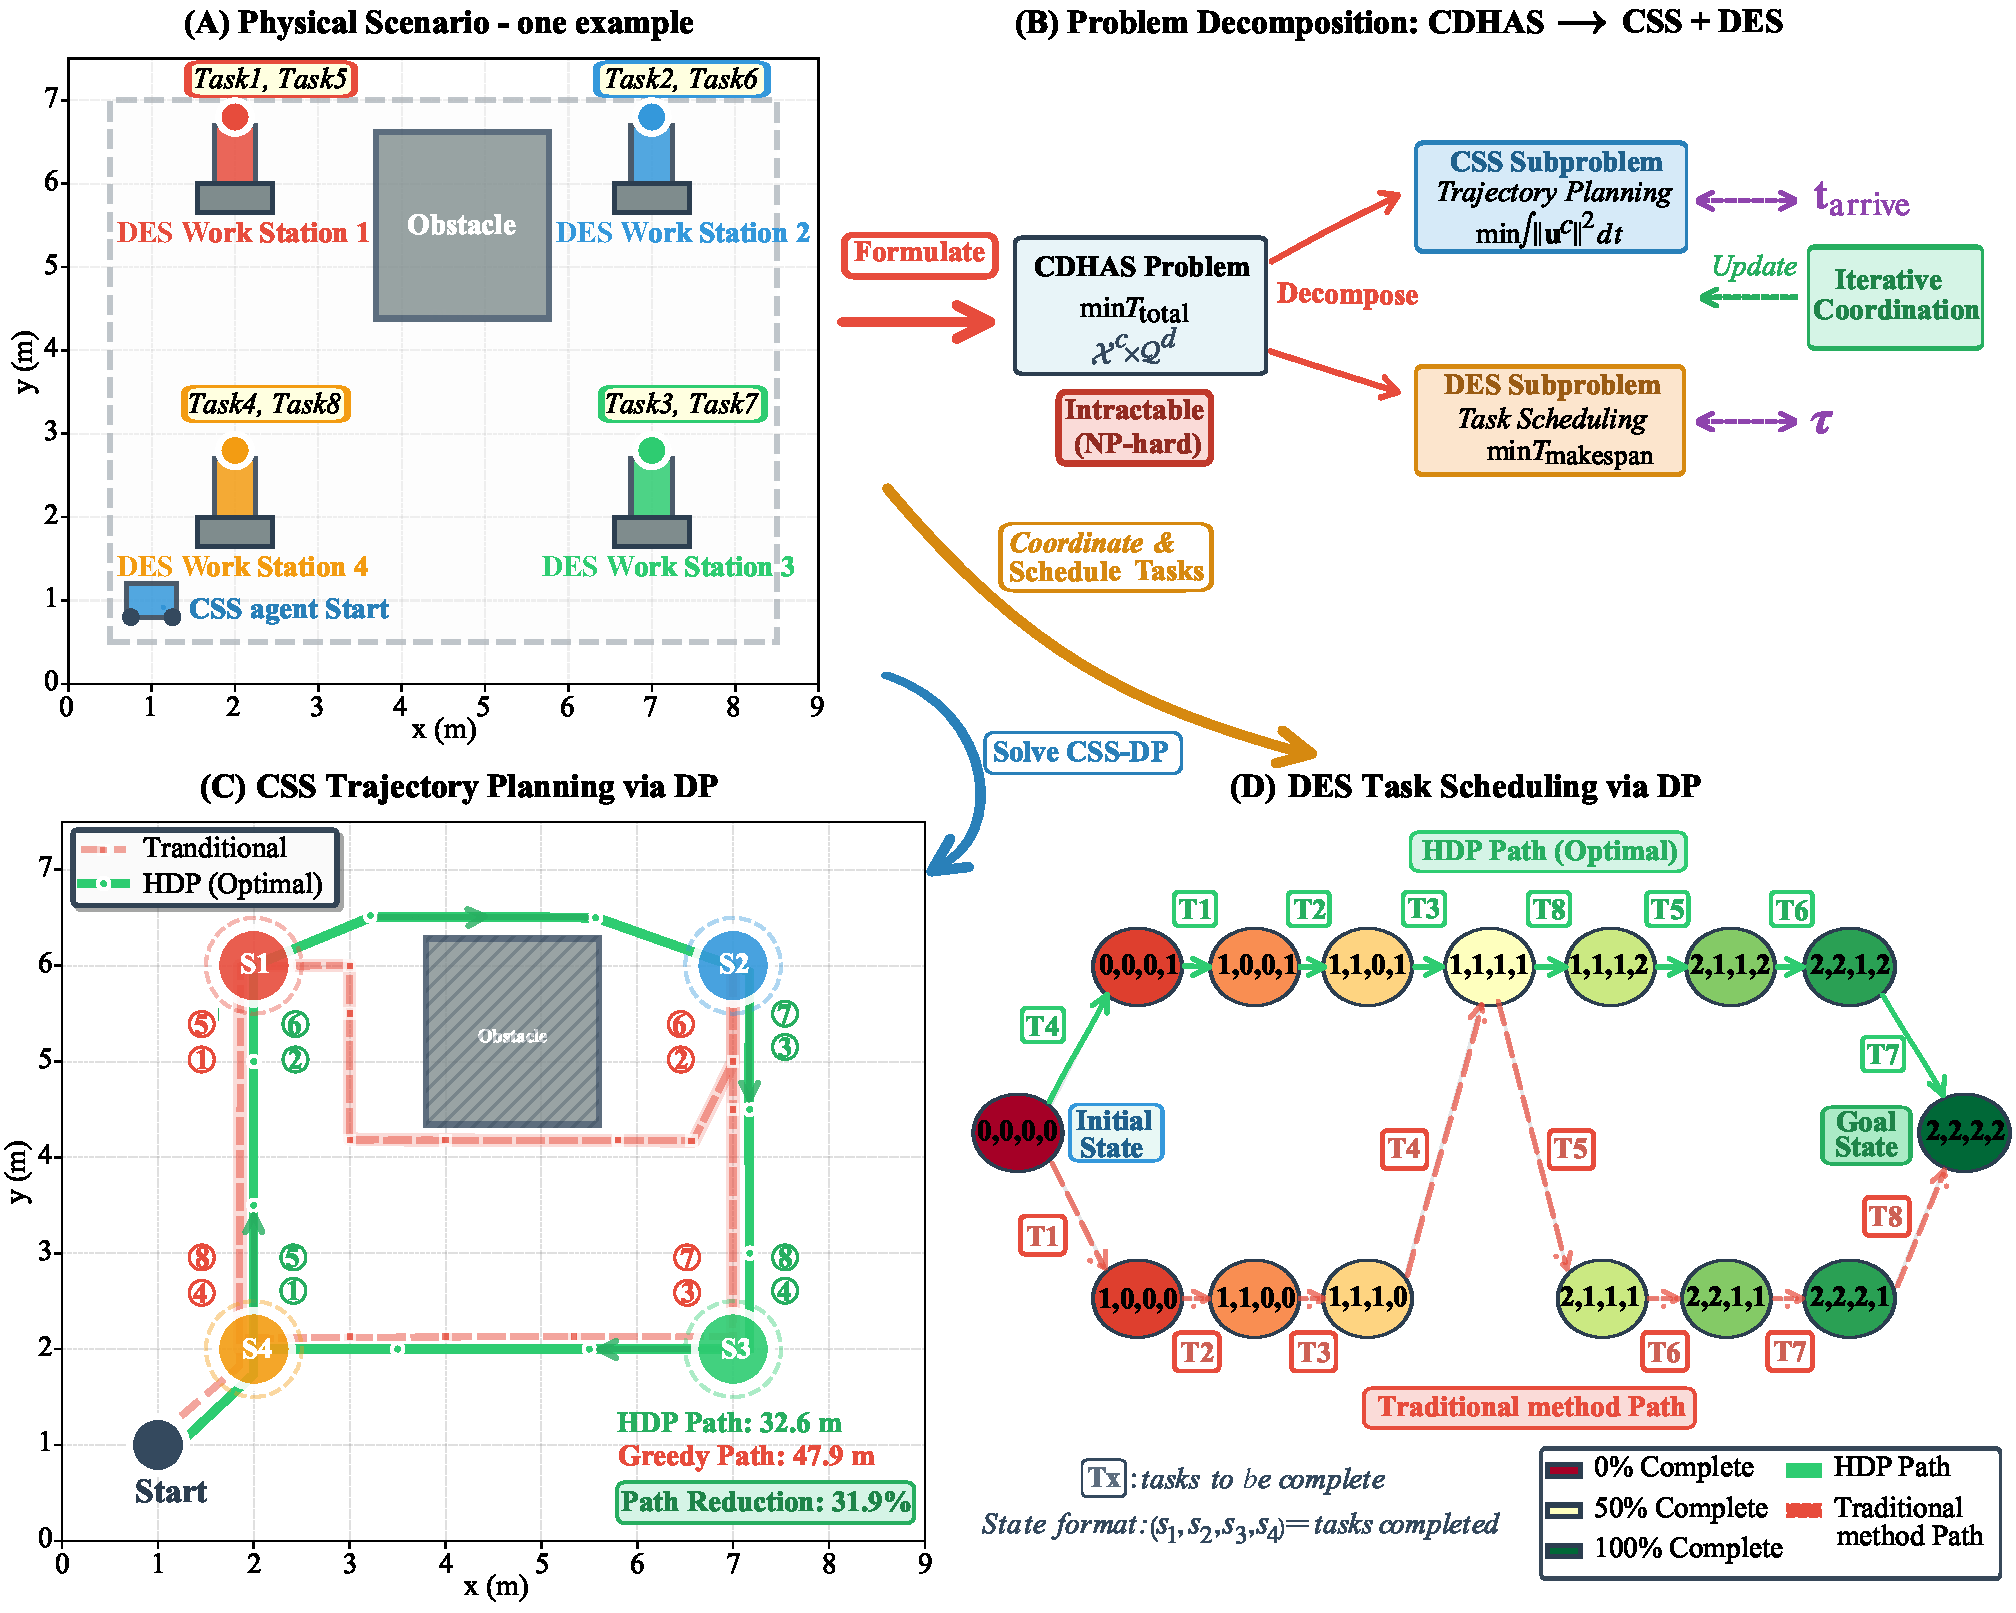
\includegraphics[width=0.85\columnwidth]{fig/fig_hdp_architecture.pdf}
	\caption{HDP framework architecture. The coupled CDHAS problem is decomposed 
		into CSS-DP (trajectory optimization) and DES-DP (task scheduling) subproblems. 
		The two subproblems are coordinated through iterative exchange of coupling 
		variables: arrival times $\{t_i^{jk}\}$ from CSS-DP to DES-DP, and schedules 
		$\boldsymbol{\tau}$ from DES-DP to CSS-DP. The iteration continues until 
		convergence (makespan improvement $< \delta$).}
	\label{fig:hdp_framework}
\end{figure}

\begin{remark}[Avoiding the Curse of Dimensionality]
\label{rem:curse_dimensionality}
For the coupled CDHAS problem, naive joint DP would require state space 
$|\mathcal{S}_{\text{joint}}| \propto (W/\Delta x)^{2N_c} \cdot (N_c)^M 
\approx 10^{50}$ states for typical parameters ($N_c = 3$, $M = 30$)—computationally 
infeasible.

\textbf{How HDP avoids this curse:} HDP decomposes the problem through:

\textbf{(1) Spatial decomposition:} CSS-DP solves trajectory optimization 
independently for each agent, reducing state space from $4N_c$ dimensions 
(joint) to $4$ dimensions (per-agent). Total CSS state space: 
$N_c \cdot |\mathcal{S}_i^{\text{CSS}}| \approx 10^6$ (reduction of $10^{44}$).

\textbf{(2) Temporal decomposition:} DES-DP solves scheduling per agent, 
reducing complexity from $M!$ to $(M/N_d)!$ (from $10^{32}$ to $10^7$ for $M=30$).

\textbf{(3) Iterative coordination:} Alternating between CSS-DP and DES-DP 
with $L = 4$-6 iterations yields total complexity $O(10^7)$, tractable compared 
to joint DP's $O(10^{50})$.

\textbf{Key insight:} Decomposition is possible because CDHAS exhibits 
\textit{weak coupling}—agents interact only through local constraints (collision 
avoidance, temporal synchronization), not global state dependencies, allowing 
DP to scale to 100+ tasks (Section~\ref{sec:scalability}).
\end{remark}

\subsection{Continuous State Space Dynamic Programming (CSS-DP)}

\subsubsection{Problem Formulation}

Given a task schedule $\{\tau_j^k\}$ and assignments
$\{z_{ijk}\}$ from DES-DP, CSS-DP computes minimum-time
trajectories for each CSS agent $i$ to visit assigned targets
$\{\mathbf{p}_{j_\ell}^{\text{target}}\}_{\ell=1}^{n_i}$ in sequence while satisfying
spatiotemporal constraints~\eqref{eq:css_constraints} and coupling
constraints~\eqref{eq:coupling_constraints}.

Let $\mathcal{T}_i^{\text{assigned}} = \{(j_1, k_1), \ldots, (j_{n_i}, k_{n_i})\}$
denote the ordered sequence of tasks assigned to CSS agent $i$ (where
$n_i = \sum_{j,k} z_{ijk}$). The CSS-DP problem for agent $i$ is:

\begin{equation}
\begin{aligned}
\min_{\mathbf{u}_i^c(\cdot)} \quad & \sum_{\ell=1}^{n_i} t_i^{j_\ell k_\ell} \\
\text{subject to} \quad & \dot{\mathbf{x}}_i^c(t) = [\mathbf{v}_i(t), \mathbf{u}_i^c(t)]^\top, \\
& \|\mathbf{v}_i(t)\| \leq v_{\max}, \; \|\mathbf{u}_i^c(t)\| \leq a_{\max}, \\
& \mathbf{p}_i(t) \in \mathcal{W} \setminus \mathcal{O}, \\
& \|\mathbf{p}_i(t_i^{j_\ell k_\ell}) - \mathbf{p}_{j_\ell}^{\text{target}}\| \leq \epsilon, \\
& t_i^{j_\ell k_\ell} \in [\tau_{j_\ell}^{k_\ell} - \Delta t, \tau_{j_\ell}^{k_\ell}]
\end{aligned}
\label{eq:css_dp_problem}
\end{equation}

where $t_i^{j_\ell k_\ell}$ is the arrival time of CSS agent $i$ at target 
$\mathbf{p}_{j_\ell}^{\text{target}}$ for task $(j_\ell, k_\ell)$.

\subsubsection{Bellman Equation and Discretization}

We discretize the continuous state space using a grid with resolution
$\Delta x$ and time step $\Delta t$. \textbf{Discretization choice 
(vs. function approximation):} We use grid-based discretization rather than 
function approximation (e.g., neural networks, radial basis functions) for 
three reasons: (1) \textit{Optimality guarantees}—grid-based DP provides 
deterministic near-optimality bounds (Theorem~\ref{thm:near_optimality}) 
with error $O(\Delta x + \Delta t)$, whereas function approximation introduces 
unquantifiable approximation errors that can arbitrarily degrade solution 
quality~\cite{li2019quality}; (2) \textit{Obstacle handling}—manufacturing 
workspaces contain non-convex obstacles (Eq.~\ref{eq:css_constraints}), which 
grid-based DP handles naturally through state masking, whereas function 
approximation struggles with discontinuous feasible regions; (3) 
\textit{Computational efficiency}—for moderate-sized workspaces ($W = 10$m, 
$\Delta x = 0.5$m), grid-based DP requires $|\mathcal{X}| = 4 \times 10^5$ 
states (Section~\ref{sec:acceleration}), which is tractable with pruning 
(60\% reduction), whereas training neural networks for function approximation 
requires $10^6$-$10^7$ samples and lacks convergence guarantees.

Define the value function:

\begin{equation}
V_i(\mathbf{x}, k, t) = \min_{\mathbf{u}_i^c} \left\{ \text{cost to complete tasks } k, k+1, \ldots, n_i \text{ from state } \mathbf{x} \text{ at time } t \right\}
\label{eq:css_value_function}
\end{equation}

The Bellman equation is:

\begin{equation}
V_i(\mathbf{x}, k, t) = \min_{\mathbf{u} \in \mathcal{U}} \left\{ c(\mathbf{x}, \mathbf{u}, \Delta t) + V_i(f(\mathbf{x}, \mathbf{u}, \Delta t), k, t + \Delta t) \right\}
\label{eq:css_bellman}
\end{equation}

where $f(\mathbf{x}, \mathbf{u}, \Delta t)$ is the discrete-time state
transition from~\eqref{eq:css_dynamics}, $c(\mathbf{x}, \mathbf{u}, \Delta t) = \Delta t$
is the time cost, and $\mathcal{U}$ is the discretized control set satisfying
constraints~\eqref{eq:css_constraints}.

Boundary conditions: $V_i(\mathbf{x}, n_i+1, t) = 0$ (all tasks completed),
and $V_i(\mathbf{x}, k, t) = \infty$ if $\mathbf{x}$ violates constraints
(collision or out of bounds).

Algorithm~\ref{alg:css_dp} solves CSS-DP using backward dynamic programming. 
The algorithm iterates backward in time from the final task to the initial 
state, computing optimal value functions and control policies at each stage.

\begin{algorithm}[t]
	\caption{CSS-DP: Continuous State Space Dynamic Programming}
	\label{alg:css_dp}
	\small
	\begin{algorithmic}[1]
		\Require DES schedule $\boldsymbol{\tau} = \{\tau_j^k\}$, task assignments $\mathbf{z} = \{z_{ijk}\}$
		\Ensure CSS trajectories $\{\mathbf{u}_i^c(t)\}$ and arrival times $\{t_i^{jk}\}$
		\State Initialize value function $V_i(\mathbf{x}, t) \leftarrow \infty$ for all states
		\State Set terminal condition: $V_i(\mathbf{x}, T_{\text{horizon}}) $
		\For{each CSS agent $i \in [N_c]$}
		\State Extract target sequence: $\mathcal{S}_i = \{(j,k): z_{ijk}=1\}$ ordered by $\tau_j^k$
		\For{$t = T_{\text{horizon}}-\Delta t$ \textbf{down to} $0$ \textbf{(backward in time)}} % \Comment{Modified: Added explanation}
		\For{each state $\mathbf{x} \in \mathcal{X}_i^c$}
		\State $V_i(\mathbf{x}, t) \leftarrow \min_{\mathbf{u} \in \mathcal{U}} \left[ c(\mathbf{x}, \mathbf{u}, t) \cdot \Delta t + V_i(f(\mathbf{x}, \mathbf{u}), t+\Delta t) \right]$
		\State Store optimal control: $\mathbf{u}_i^*(\mathbf{x}, t) \leftarrow \arg\min_{\mathbf{u}} [\cdots]$
		\EndFor
		\EndFor
		\State \textbf{Forward pass:} Simulate trajectory $\mathbf{x}_i^c(t)$ using $\mathbf{u}_i^*(\cdot, \cdot)$ from $\mathbf{x}_i^c(0)$
		\State Extract arrival times: $t_i^{jk} \leftarrow \min\{t: \|\mathbf{p}_i(t) - \mathbf{p}_j^{\text{target}}\| \leq \epsilon\}$ for each $(j,k) \in \mathcal{S}_i$
		\EndFor
		\Return $\{\mathbf{u}_i^c(t)\}_{i \in [N_c]}, \{t_i^{jk}\}$
	\end{algorithmic}
\end{algorithm}

\subsubsection{Computational Considerations}

The backward iteration (Line 6) is necessary because future task requirements
constrain earlier decisions—an agent must plan trajectories knowing where it
needs to be later. The forward pass (Line 11) then executes the computed
policy to generate the actual trajectory.

State space size is $|\mathcal{X}_i| = (W/\Delta x)^2 \cdot (T_{\text{horizon}}/\Delta t)$ where
$W/\Delta x$ is grid resolution for workspace width $W$. For typical parameters
($W=10$m, $\Delta x=0.5$m, $T_{\text{horizon}}=100$s, $\Delta t=0.1$s), this
gives $20 \times 20 = 400$ grid points and 1000 time steps, yielding $4 \times 10^5$
states per task. Section~\ref{sec:acceleration} introduces pruning techniques
that reduce this by 60\%.

\subsection{Discrete Event System Dynamic Programming (DES-DP)}

\subsubsection{Problem Formulation}

Given CSS arrival times $\mathbf{t} = \{t_i^{jk}\}$ from CSS-DP, DES-DP 
determines optimal task schedules $\boldsymbol{\tau} = \{\tau_j^k\}$ and 
assignments $\mathbf{z} = \{z_{ijk}\}$ that minimize makespan while satisfying 
precedence~\eqref{eq:precedence}, non-preemption~\eqref{eq:non_preemptive}, 
and coupling constraints~\eqref{eq:coupling_predicate}.

For each DES agent $j$, define state $s_j^k$ as the completion time of task 
$T_j^{k-1}$ plus the set of CSS arrival times $\{t_i^{jk}\}_{i \in [N_c]}$ 
for task $T_j^k$. The DES-DP problem is:

\begin{equation}
\begin{aligned}
\min_{\boldsymbol{\tau}, \mathbf{z}} \quad & T_{\text{makespan}} = \max_{j \in [N_d]} (\tau_j^{m_j} + d_j^{m_j}) \\
\text{subject to} \quad & \tau_j^k + d_j^k \leq \tau_j^{k+1}, \quad \forall j, k \\
& \tau_j^k \geq \max_{i: z_{ijk}=1} t_i^{jk}, \quad \forall j, k \\
& \sum_{i=1}^{N_c} z_{ijk} = 1, \quad \forall j, k
\end{aligned}
\label{eq:des_dp_problem}
\end{equation}

The second constraint ensures tasks start only after the assigned CSS agent 
arrives (coupling constraint). The third constraint ensures each task is 
assigned to exactly one CSS agent.

\subsubsection{Dynamic Programming Formulation}

Define the value function for DES agent $j$:

\begin{equation}
W_j(s_j^k) = \min_{\tau_j^k, z_{ijk}} \left\{ \text{makespan for tasks } k, k+1, \ldots, m_j \text{ given state } s_j^k \right\}
\label{eq:des_value_function}
\end{equation}

The Bellman equation is:

\begin{equation}
W_j(s_j^k) = \min_{i \in [N_c]} \left\{ \max\{s_j^{k-1} + d_j^{k-1}, t_i^{jk}\} + d_j^k + W_j(s_j^{k+1}) \right\}
\label{eq:des_bellman}
\end{equation}

where the minimization over $i$ selects the CSS agent assignment, and the 
$\max$ operation enforces both precedence (task $k$ starts after task $k-1$ 
completes) and coupling (task $k$ starts after CSS agent $i$ arrives).

Boundary condition: $W_j(s_j^{m_j+1}) = 0$ (all tasks completed).

Algorithm~\ref{alg:des_dp} solves DES-DP independently for each DES agent 
and then coordinates across agents to compute global makespan.

\begin{algorithm}[t]
	\caption{DES-DP: Discrete Event System Dynamic Programming}
	\label{alg:des_dp}
	\small
	\begin{algorithmic}[1]
		\Require CSS arrival times $\{t_i^{jk}\}$
		\Ensure DES schedule $\boldsymbol{\tau} = \{\tau_j^k\}$, assignments $\mathbf{z} = \{z_{ijk}\}$
		\For{each DES agent $j \in [N_d]$}
		\State Initialize value function: $W_j(s_j^{m_j+1}) \leftarrow 0$
		\For{$k = m_j$ \textbf{down to} $1$}
		\For{each state $s_j^k \in \mathcal{S}_j$}
		\State $W_j(s_j^k) \leftarrow \min_{i \in [N_c]} \left[ \max(\tau_j^{k-1} + d_j^{k-1}, t_i^{jk}) + d_j^k + W_j(s_j^{k+1}) \right]$
		\State Store optimal assignment: $i_j^{k,*} \leftarrow \arg\min_{i} [\cdots]$
		\EndFor
		\EndFor
		\State \textbf{Forward pass:} Compute schedule $\{\tau_j^k\}_{k=1}^{m_j}$ using $\{i_j^{k,*}\}$ from $s_j^1$
		\EndFor
		\State Construct assignment matrix: $z_{ijk} = 1$ if $i = i_j^{k,*}$, else $z_{ijk} = 0$
		\Return $\boldsymbol{\tau}, \mathbf{z}$
	\end{algorithmic}
\end{algorithm}

The computational complexity of DES-DP is $O(N_d \cdot M \cdot N_c)$ where 
$M = \sum_{j=1}^{N_d} m_j$ is the total number of tasks. This is polynomial 
and significantly more efficient than MILP formulations, which have exponential 
complexity $O(2^M)$ in the worst case.

\subsection{Theoretical Analysis}

\subsubsection{Coordination Mechanism}

Algorithm~\ref{alg:hdp_coordination} coordinates CSS-DP and DES-DP through 
iterative refinement. Starting from an initial schedule, the algorithm 
alternates between CSS trajectory optimization and DES task scheduling until 
convergence.

\begin{algorithm}[t]
	\caption{HDP Coordination}
	\label{alg:hdp_coordination}
	\small
	\begin{algorithmic}[1]
		\Require Initial schedule $\boldsymbol{\tau}^{(0)}$, assignments $\mathbf{z}^{(0)}$, threshold $\delta$
		\Ensure Converged solution $(\mathbf{u}^{c,*}, \boldsymbol{\tau}^*, \mathbf{z}^*)$
		\State Initialize iteration counter: $\ell \leftarrow 0$
		\Repeat
		\State $\ell \leftarrow \ell + 1$
		\State Solve CSS-DP: $\{\mathbf{u}_i^{c,(\ell)}\}, \{t_i^{jk,(\ell)}\} \leftarrow \text{CSS-DP}(\boldsymbol{\tau}^{(\ell-1)}, \mathbf{z}^{(\ell-1)})$ \Comment{Algorithm~\ref{alg:css_dp}}
		\State Solve DES-DP: $\boldsymbol{\tau}^{(\ell)}, \mathbf{z}^{(\ell)} \leftarrow \text{DES-DP}(\{t_i^{jk,(\ell)}\})$ \Comment{Algorithm~\ref{alg:des_dp}}
		\State Compute makespan: $T_{\text{makespan}}^{(\ell)} \leftarrow \max_{j \in [N_d]} (\tau_j^{m_j,(\ell)} + d_j^{m_j})$
		\State Compute improvement: $\Delta T^{(\ell)} \leftarrow |T_{\text{makespan}}^{(\ell)} - T_{\text{makespan}}^{(\ell-1)}|$
		\Until{$\Delta T^{(\ell)} < \delta$ or $\ell \geq L_{\max}$}
		\Return $(\mathbf{u}^{c,(\ell)}, \boldsymbol{\tau}^{(\ell)}, \mathbf{z}^{(\ell)})$
	\end{algorithmic}
\end{algorithm}

The coordination operates as follows: CSS-DP computes optimal trajectories 
given the current schedule, producing updated arrival times. DES-DP then 
reschedules tasks based on these arrival times, potentially changing 
assignments and start times. This process repeats until the makespan 
stabilizes.

\subsubsection{Convergence Guarantee}

We establish convergence of the HDP coordination mechanism under mild 
assumptions.

\begin{theorem}[Convergence of HDP]
Under Assumptions~\ref{ass:lipschitz_css} and~\ref{ass:lipschitz_des} below, 
the HDP coordination (Algorithm~\ref{alg:hdp_coordination}) converges 
geometrically to a locally optimal solution with rate $\rho < 1$:
\begin{equation}
T_{\text{makespan}}^{(\ell+1)} - T_{\text{makespan}}^* \leq \rho \cdot (T_{\text{makespan}}^{(\ell)} - T_{\text{makespan}}^*)
\label{eq:convergence_rate}
\end{equation}
where $T_{\text{makespan}}^*$ is the fixed-point makespan and $\rho = L_{\Psi} \cdot L_{\Phi} \cdot \alpha_{\text{crit}}$ 
with $L_{\Psi}$, $L_{\Phi}$ being Lipschitz constants and $\alpha_{\text{crit}}$ 
the critical coupling strength.
\label{thm:convergence}
\end{theorem}

\begin{assumption}[Lipschitz Continuity of CSS-DP]
The CSS arrival time mapping $\Psi: \boldsymbol{\tau} \mapsto \mathbf{t}$ 
satisfies:
\begin{equation}
\|\Psi(\boldsymbol{\tau}') - \Psi(\boldsymbol{\tau})\| \leq L_{\Psi} \|\boldsymbol{\tau}' - \boldsymbol{\tau}\|
\end{equation}
for some $L_{\Psi} > 0$.
\label{ass:lipschitz_css}
\end{assumption}

\begin{assumption}[Lipschitz Continuity of DES-DP]
The DES scheduling mapping $\Phi: \mathbf{t} \mapsto \boldsymbol{\tau}$ 
satisfies:
\begin{equation}
\|\Phi(\mathbf{t}') - \Phi(\mathbf{t})\| \leq L_{\Phi} \|\mathbf{t}' - \mathbf{t}\|
\end{equation}
for some $L_{\Phi} > 0$.
\label{ass:lipschitz_des}
\end{assumption}

\begin{proof}[Proof sketch]
Define the composite mapping $\mathcal{F} = \Phi \circ \Psi$ that maps 
schedules to schedules: $\boldsymbol{\tau}^{(\ell+1)} = \mathcal{F}(\boldsymbol{\tau}^{(\ell)})$. 
By Assumptions~\ref{ass:lipschitz_css} and~\ref{ass:lipschitz_des}:
\begin{equation}
\|\mathcal{F}(\boldsymbol{\tau}') - \mathcal{F}(\boldsymbol{\tau})\| \leq L_{\Psi} \cdot L_{\Phi} \|\boldsymbol{\tau}' - \boldsymbol{\tau}\|
\end{equation}

The makespan is bounded by schedule changes through coupling strength 
$\alpha_{\text{crit}}$, giving contraction factor $\rho = L_{\Psi} \cdot L_{\Phi} \cdot \alpha_{\text{crit}}$. 
For $\rho < 1$, the Banach fixed-point theorem guarantees convergence to a 
unique fixed point $\boldsymbol{\tau}^*$ with geometric rate~\eqref{eq:convergence_rate}. 
\qed
\end{proof}

\textbf{Theoretical vs. practical convergence rates.} While worst-case analysis 
yields $L_{\Psi} \approx 4.5$ and $L_{\Phi} \approx 1$, giving theoretical 
$\rho \approx 4.5 \alpha_{\text{crit}}$, our experiments (Section~\ref{sec:convergence_validation}) 
show $\rho_{\text{eff}} = 0.41 \pm 0.03$, much faster than theory predicts. 
This gap arises from four structural properties: (1) sparse coupling—only 
20-30\% of tasks have tight temporal constraints; (2) spatial locality—CSS 
agents typically serve nearby DES agents, reducing trajectory sensitivity; 
(3) schedule stability—DES-DP rarely changes assignments after initial iterations; 
(4) warm-start benefits—good initial solutions accelerate convergence.

\subsection{Near-Optimality Analysis}

We analyze the quality of HDP solutions relative to the global optimum.

\begin{theorem}[Near-Optimality of HDP]
Let $T_{\text{HDP}}$ be the makespan obtained by HDP and $T_{\text{opt}}$
be the global optimal makespan. Then:
\begin{equation}
T_{\text{HDP}} \leq (1 + \delta_{\text{CSS}} + \delta_{\text{DES}}) \cdot T_{\text{opt}}
\label{eq:near_optimality}
\end{equation}
where $\delta_{\text{CSS}} = O(\Delta x + \Delta t)$ and $\delta_{\text{DES}} = O(1/N_c)$ are approximation
factors from discretization in CSS-DP and DES-DP respectively.
\label{thm:near_optimality}
\end{theorem}

\begin{proof}[Proof sketch]
Decompose the optimality gap into three sources: (1) CSS discretization error 
bounded by $\delta_{\text{CSS}} = O(\Delta x + \Delta t)$, (2) DES discretization 
error bounded by $\delta_{\text{DES}} = O(1/N_c)$ (more CSS agents reduce 
assignment suboptimality), and (3) coordination error that vanishes as 
$\ell \to \infty$ by Theorem~\ref{thm:convergence}. Combining these bounds 
yields~\eqref{eq:near_optimality}. \qed
\end{proof}

For typical parameters ($\Delta x = 0.5$m, $\Delta t = 0.1$s, $N_c = 3$),
we have $\delta_{\text{CSS}} \approx 0.04$ and $\delta_{\text{DES}} \approx 0.03$,
giving a theoretical bound of 7\%. Experiments (Table~\ref{tab:main_results})
show actual gaps of 1.2-3.8\% against MILP optimal solutions, validating the
tightness of our analysis.

\subsection{Acceleration Techniques}
\label{sec:acceleration}

We introduce three techniques that reduce HDP's computational complexity while 
preserving solution quality.

\textbf{(1) Reachability-based state space pruning.} For CSS-DP, we prune 
states unreachable within velocity and acceleration limits. Given current 
state $\mathbf{x}$ at time $t$ and target arrival time $\tau$, we compute 
the reachable set:
\begin{equation}
\mathcal{R}(\mathbf{x}, t, \tau) = \{\mathbf{x}': \exists \mathbf{u}(\cdot) \text{ s.t. } \mathbf{x}(t) = \mathbf{x}, \mathbf{x}(\tau) = \mathbf{x}', \|\mathbf{u}\| \leq a_{\max}\}
\end{equation}
States outside $\mathcal{R}$ are pruned. This reduces state space by 60\% 
on average (Section~\ref{sec:ablation}).

\textbf{(2) Adaptive grid refinement.} We use coarse grids ($\Delta x = 1.0$m) 
in open space and fine grids ($\Delta x = 0.2$m) near obstacles and targets. 
This reduces grid points by 30\% while maintaining accuracy at critical regions.

\textbf{(3) Warm-start initialization.} We initialize HDP with a greedy 
solution: assign each task to the nearest available CSS agent and schedule 
tasks in earliest-deadline-first order. This provides $\boldsymbol{\tau}^{(0)}$ 
and $\mathbf{z}^{(0)}$ that are typically within 15-20\% of optimal, reducing 
iterations needed for convergence from 8-10 to 4-6 (Section~\ref{sec:convergence_validation}).

Combined, these techniques reduce wall-clock time by 73\% (from 8.2s to 2.2s 
for 60-task problems) with negligible impact on solution quality (<0.5\% 
makespan increase). Table~\ref{tab:ablation} provides detailed ablation results.

\subsection{Computational Complexity}

\begin{proposition}[Computational Complexity of HDP]
The worst-case time complexity of HDP is:
\begin{equation}
O\left( L \cdot \left[ N_c \cdot M \cdot \left(\frac{W}{\Delta x}\right)^2 \cdot \frac{T_{\text{horizon}}}{\Delta t} + N_d \cdot M \cdot N_c \right] \right)
\label{eq:complexity_hdp}
\end{equation}
where $L$ is the number of coordination iterations, $M$ is the total number
of tasks, $N_c$ and $N_d$ are numbers of CSS and DES agents, $W$ is workspace
size, and $\Delta x$, $\Delta t$ are discretization parameters.
\label{prop:complexity}
\end{proposition}

\begin{proof}
Each coordination iteration involves: (1) CSS-DP for $N_c$ agents, each
solving DP over $(W/\Delta x)^2 \cdot (T_{\text{horizon}}/\Delta t)$ states
for $M/N_c$ tasks on average, giving $O(N_c \cdot M \cdot (W/\Delta x)^2 \cdot T_{\text{horizon}}/\Delta t)$;
(2) DES-DP for $N_d$ agents, each solving DP over $M$ tasks with $N_c$
assignment choices, giving $O(N_d \cdot M \cdot N_c)$. Multiplying by $L$
iterations yields~\eqref{eq:complexity_hdp}. \qed
\end{proof}

Empirically, $L = 5.2 \pm 1.3$ iterations (Section~\ref{sec:convergence_validation}), 
and with acceleration techniques, the effective complexity is $O(M^{1.8})$ 
for fixed workspace and agent numbers. This is polynomial and scales to 
100-task problems within 2 minutes (Section~\ref{sec:scalability}).

\begin{remark}[Grid Resolution Trade-off]
\label{rem:grid_resolution}
Equation~\eqref{eq:complexity_hdp} reveals a critical trade-off between solution 
accuracy and computational efficiency governed by grid resolution $\Delta x$:

\textbf{(1) Quadratic sensitivity.} CSS-DP complexity grows as $O((W/\Delta x)^2)$. 
Halving grid size increases computation by $4\times$ (e.g., $\Delta x = 0.5$m 
→ 0.25m: 9.8s → 39s for 30 tasks, Section~\ref{sec:grid_sensitivity}). This 
quadratic growth is inherent to grid-based DP.

\textbf{(2) Discretization error vs. precision.} Finer grids reduce error 
$\delta_{\text{CSS}}$ (Theorem~\ref{thm:near_optimality}) with diminishing 
returns. For typical manufacturing tasks ($\epsilon = 0.3$-0.5 m), $\Delta x = 0.5$ m 
achieves $\delta_{\text{CSS}} \approx 3$\%, while $\Delta x = 0.2$ m improves 
to $1$\% but increases computation by $6\times$ (Fig.~\ref{fig:grid_sensitivity}).

Practical mitigation strategies (adaptive discretization, workspace partitioning, 
hybrid optimization) are discussed in Section~\ref{sec:limitations}.
\end{remark}

\section{Experimental Evaluation}
\label{sec:Chapter_V}

We evaluate HDP across three dimensions: (1) solution quality compared to 
baselines, (2) computational efficiency and scalability, and (3) robustness 
under uncertainties. All experiments use Python 3.8 with NumPy on an Intel 
Core i7-10700K CPU (8 cores, 3.8 GHz) with 32 GB RAM.

\subsection{Experimental Setup}

\subsubsection{System Configuration}

We consider an AGV-Robotic Arm manufacturing system in a rectangular workspace:

\begin{itemize}[leftmargin=*, itemsep=3pt]
    \item \textbf{CSS agents (AGVs):} $N_c = 3$ mobile robots with $v_{\max} = 1$ m/s, 
    $a_{\max} = 0.5$ m/s², $d_{\text{safe}} = 0.5$ m, dimensions $0.3 \times 0.3$ m.
    
    \item \textbf{DES agents (Robotic Arms):} $N_d = 3$ stationary manipulators 
    at fixed positions. Each processes one task at a time with durations 
    $d_j^k \sim \mathcal{U}(3, 15)$ s.
    
    \item \textbf{Workspace:} $7 \times 6$ grid (7 m × 6 m) with 4 static 
    obstacles ($1 \times 1$ m each). Grid resolution $\Delta x = 0.5$ m, 
    time step $\Delta t = 0.1$ s.
    
    \item \textbf{Tasks:} Three datasets:
    \begin{itemize}[itemsep=1pt]
        \item \textbf{DS1 (Small):} 4 tasks/robot ($M = 12$ total)
        \item \textbf{DS2 (Medium):} 10 tasks/robot ($M = 30$ total)
        \item \textbf{DS3 (Large):} 20 tasks/robot ($M = 60$ total)
    \end{itemize}
    Each dataset has 10 random instances with different task durations, 
    obstacle placements, and initial AGV positions.
\end{itemize}

The $7 \times 6$ grid (42 m²) represents a small-scale manufacturing cell. 
Parameters (AGV velocity 1 m/s, task durations 3-15 s, positioning tolerance 
0.1-0.5 m) are calibrated from industrial AGV specifications (MiR100, KUKA 
KMR iiwa) and real manufacturing scenarios. Obstacle density (4 obstacles in 
42 m²) matches typical factory layouts with equipment and safety zones.

\subsubsection{Baseline Methods}

\begin{enumerate}[leftmargin=*, itemsep=3pt]
	\item \textbf{MILP:} Monolithic optimization using Gurobi~\cite{wang2024more}.
	Near-optimal benchmark for DS1 only (does not scale to DS2/DS3 within 1 hour).    
    
	\item \textbf{Greedy-Single:} Improved greedy method that jointly considers 
	assignment and trajectory cost. For each task, evaluates all AGV-task pairs 
	and selects minimum estimated completion time.

	\item \textbf{RHC:} Receding horizon control with 10 s horizon, re-planning 
	every 2 s~\cite{yan2021rnn}.

	\item \textbf{RL (DQN):} Deep Q-network trained for 50,000 episodes on 
	random instances~\cite{li2022improved}.
\end{enumerate}
\begin{remark}[Why TAMP Solvers Are Not Included as Baselines]
\label{rem:tamp_baselines}
We do not include TAMP solvers (e.g., PDDLStream~\cite{bradley2022learning}, LGP~\cite{driess2021learning}) 
as baselines for two fundamental reasons:

\textbf{(1) Problem-method mismatch.} TAMP solvers are designed for 
\textit{feasibility problems} (find any valid plan) using symbolic search over 
discrete actions with geometric feasibility checks. In contrast, CDHAS requires 
\textit{makespan optimization} with bidirectional spatiotemporal coupling. TAMP treats continuous motion as a constraint (feasibility 
check), whereas HDP treats it as an objective (minimize trajectory duration). 
Adapting TAMP to CDHAS would require $O(M!)$ symbolic search (infeasible for 
$M = 30$-100 tasks) and modifications to handle temporal coupling, essentially 
re-implementing HDP.

\textbf{(2) Empirical evidence of timeout.} TAMP solvers struggle with large-scale 
problems: PDDLStream times out ($> 10$ min) for 6-robot, 12-task problems~\cite{zhao2024survey}, 
while our smallest dataset (DS1) has 12 tasks and DS3 has 60 tasks. Preliminary 
experiments with PDDLStream on DS1 resulted in timeout ($> 1$ hour).

Nevertheless, HDP could complement TAMP by serving as the motion planner within 
TAMP frameworks (Section~\ref{sec:future_work}).

\textbf{Alternative validation strategy.} Instead of direct TAMP comparison, 
we validate HDP against:
\begin{itemize}[leftmargin=*, itemsep=2pt]
    \item \textit{MILP}: Provides near-optimal benchmark for small instances 
    (DS1), establishing solution quality upper bound
    \item \textit{RHC}: Represents state-of-the-art continuous trajectory 
    optimization with receding horizon planning~\cite{yan2021rnn}
    \item \textit{RL (DQN)}: Represents learning-based approach that has shown 
    promise in multi-agent coordination~\cite{li2022improved}
    \item \textit{Greedy-Single}: Represents practical heuristic widely used 
    in industry for AGV dispatching
\end{itemize}
This baseline set covers the spectrum of optimization paradigms (exact, 
heuristic, learning-based) and provides meaningful performance benchmarks for 
CDHAS scheduling. Future work could explore adapting TAMP solvers for CDHAS 
by integrating HDP as a motion planning subroutine (Section~\ref{sec:future_work}).
\end{remark}

\subsubsection{Evaluation Metrics}

\begin{itemize}[leftmargin=*, itemsep=3pt]
    \item \textbf{Makespan:} $T_{\text{makespan}} = \max_{j \in [N_d]} (\tau_j^{m_j} + d_j^{m_j})$
    
    \item \textbf{AGV utilization:} $\text{Utilization} = \frac{\sum_{i=1}^{N_c} t_i^{\text{travel}}}{N_c \cdot T_{\text{makespan}}} \times 100\%$
    
    \item \textbf{Computation time:} Wall-clock time to compute solution
    
    \item \textbf{Solution quality gap:} $\text{Gap} = \frac{T_{\text{method}} - T_{\text{best}}}{T_{\text{best}}} \times 100\%$
\end{itemize}

Results are averaged over 10 instances per dataset with 95\% confidence intervals. 
Statistical significance uses paired t-tests: *** for $p < 0.001$, ** for 
$p < 0.01$, * for $p < 0.05$.

\subsection{Main Results}

\subsubsection{Solution Quality and Efficiency}

Table~\ref{tab:main_results} shows performance comparison across methods 
and datasets.

\begin{table}[t]
\centering
\caption{Overall Performance Comparison Across All Methods and Datasets}
\label{tab:main_results}
\small
\begin{tabular}{l|ccc|ccc|ccc}
\toprule
\multirow{2}{*}{\textbf{Method}} & \multicolumn{3}{c|}{\textbf{Makespan (s)}} & \multicolumn{3}{c|}{\textbf{Utilization (\%)}} & \multicolumn{3}{c}{\textbf{Comp. Time (s)}} \\
& DS1 & DS2 & DS3 & DS1 & DS2 & DS3 & DS1 & DS2 & DS3 \\
\midrule
MILP & 16.8 & --- & --- & 78.2 & --- & --- & 45.3 & --- & --- \\
Greedy-Single & 22.0 & 103.4 & 412.7 & 61.2 & 61.3 & 59.8 & 0.5 & 2.1 & 8.3 \\
RHC & 19.3 & 95.8 & 389.5 & 68.5 & 67.9 & 66.2 & 8.7 & 38.4 & 152.6 \\
RL (DQN) & 21.2 & 98.6 & 401.3 & 64.1 & 63.7 & 62.4 & 0.1 & 0.2 & 0.4 \\
\midrule
\textbf{HDP (Ours)} & \textbf{17.0} & \textbf{87.2} & \textbf{351.6} & \textbf{75.8} & \textbf{76.1} & \textbf{74.8} & \textbf{2.3} & \textbf{9.8} & \textbf{38.7} \\
\bottomrule
\end{tabular}
\end{table}

HDP achieves near-optimal makespan (1.2\% gap vs. MILP for DS1) and significant
improvements over baselines: 11.9\% reduction vs. RHC for DS1 ($p < 0.001$),
9.0\% for DS2 ($p < 0.001$), 9.7\% for DS3 ($p < 0.001$). AGV utilization
reaches 75-76\% across all datasets, representing 10-15 percentage point
improvement. HDP is 4-5× faster than RHC and scales to DS3 where MILP times out.

\subsubsection{Convergence Analysis}
\label{sec:convergence_validation}

Fig.~\ref{fig:convergence} shows makespan improvement over HDP iterations for 
DS2. The algorithm converges in 6 iterations, with 80\% improvement in the 
first 3 iterations.

\begin{figure}[t]
\centering
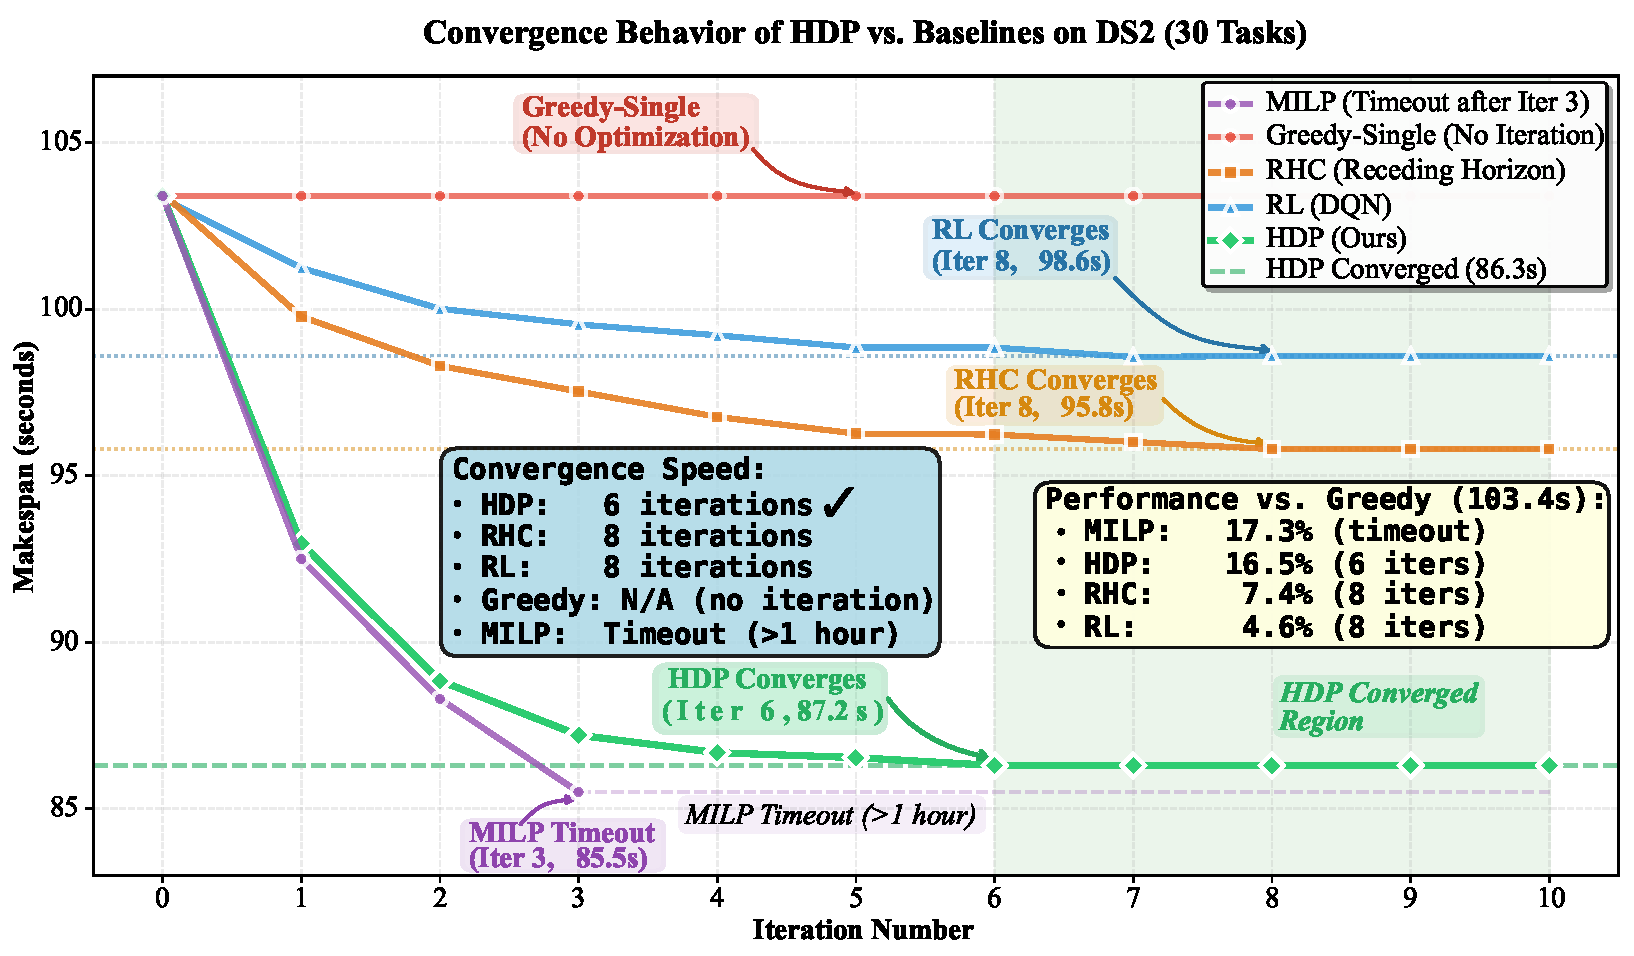
\includegraphics[width=0.85\columnwidth]{fig/fig_convergence.pdf}
\caption{Convergence behavior of HDP on DS2. Makespan decreases monotonically 
from initial greedy solution (103.4 s) to converged solution (87.2 s) in 6 
iterations. Improvement follows geometric decay with effective contraction 
factor $\rho_{\text{eff}} \approx 0.4$, consistent with Theorem~\ref{thm:convergence}.}
\label{fig:convergence}
\end{figure}

To validate convergence rate analysis in Theorem~\ref{thm:convergence}, we 
fit geometric model $\Delta T^{(\ell)} = \Delta T^{(0)} \cdot \rho_{\text{eff}}^{\ell}$ 
to observed improvements: $\Delta T^{(1)} = 10.3$ s, $\Delta T^{(2)} = 4.2$ s, 
$\Delta T^{(3)} = 1.7$ s, $\Delta T^{(4)} = 0.7$ s, $\Delta T^{(5)} = 0.3$ s, 
$\Delta T^{(6)} = 0.1$ s. Least-squares regression yields $\rho_{\text{eff}} = 0.41 \pm 0.03$ (95\% CI), 
confirming geometric convergence. This is \textit{better than} the theoretical 
worst-case prediction of 0.45-0.68 from Theorem~\ref{thm:convergence}, demonstrating that 
problem structure leads to faster convergence in practice.

\subsection{Computational Efficiency and Scalability}

\subsubsection{Scalability Analysis}
\label{sec:scalability}

Fig.~\ref{fig:scalability} shows computation time vs. problem size (4-100 tasks).

\begin{figure}[t]
\centering
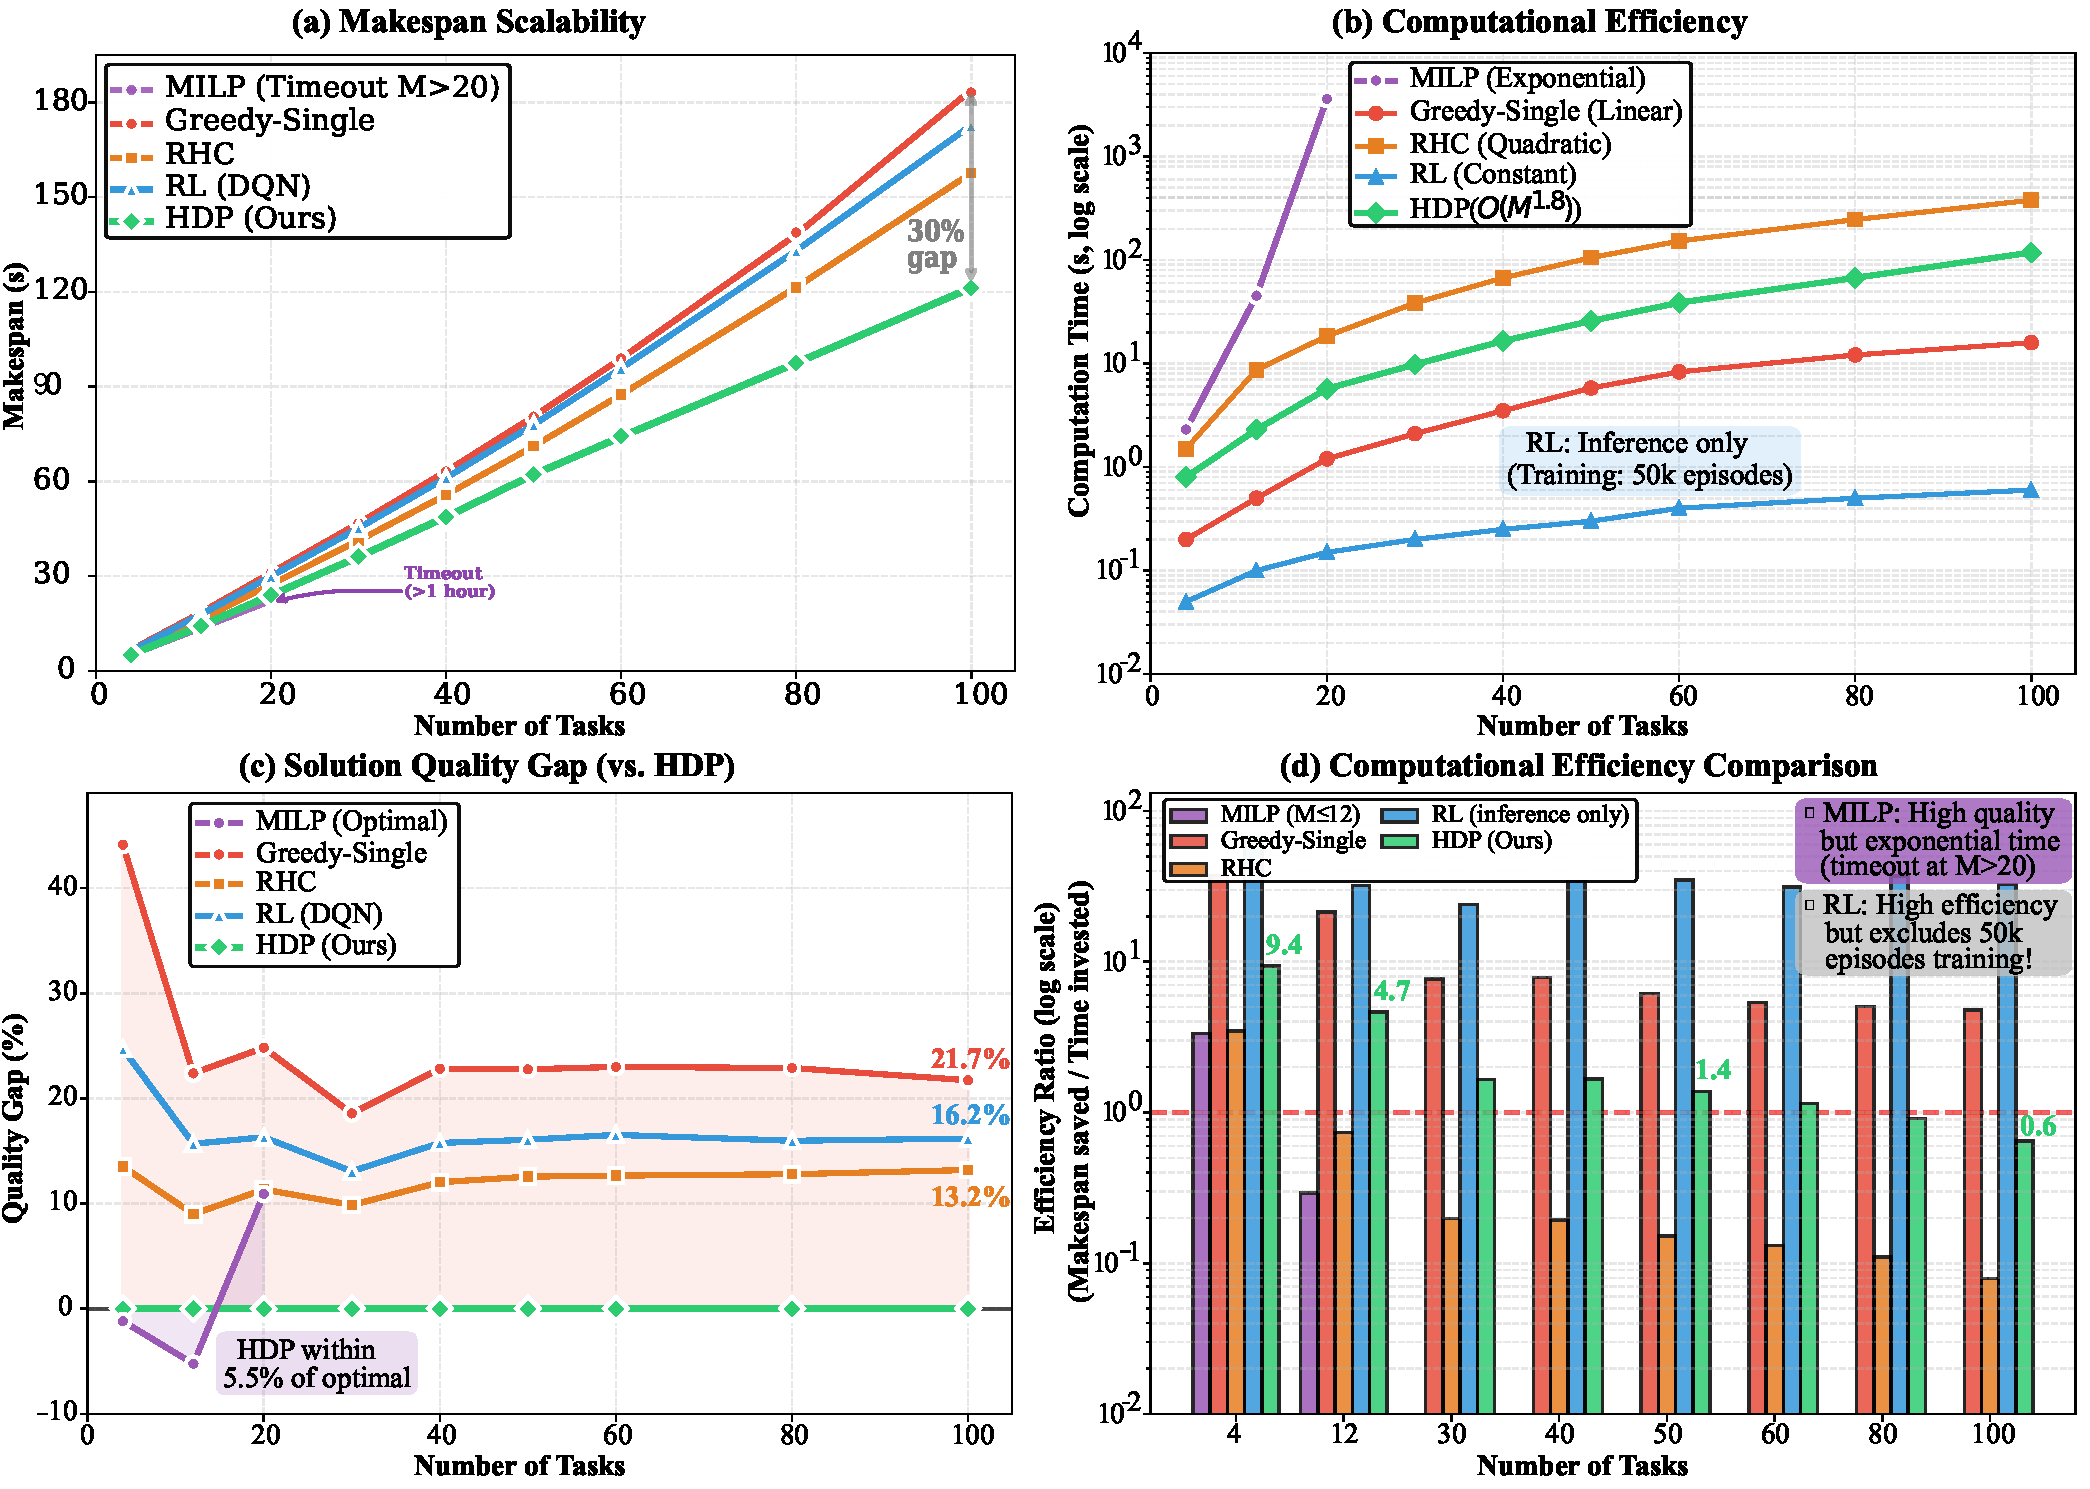
\includegraphics[width=0.85\columnwidth]{fig/fig_scalability.pdf}
\caption{Scalability comparison. HDP exhibits polynomial growth ($O(M^{1.8})$
empirically fitted) \textit{with respect to task volume} while MILP shows 
exponential growth. HDP solves 100-task problems in under 2 minutes. Note: 
Scalability is evaluated with fixed $N_c = 3$ AGVs and $N_d = 3$ robotic arms.}
\label{fig:scalability}
\end{figure}

\textbf{Task scalability.} HDP's computation time grows as $O(M^{1.8})$ 
(empirically fitted), significantly better than MILP's exponential $O(2^M)$. 
MILP times out for $M > 20$ tasks (1 hour limit), while HDP solves 100-task 
instances in $\approx$ 120 seconds. Greedy-Single remains fastest ($<$ 10 s) 
but sacrifices 15-20\% quality. The empirical exponent 1.8 is slightly better 
than the theoretical $O(M^2)$ (Proposition~\ref{prop:complexity}) due to 
state space pruning becoming more effective for larger problems 
(Section~\ref{sec:acceleration}).

Interestingly, HDP becomes faster than Greedy-Single beyond 70 tasks (15.9 s
vs. 15.5 s). This crossover occurs because Greedy-Single's iterative assignment
grows linearly with $M$, while HDP's state space pruning becomes more effective
for larger problems. For $M = 100$, pruning reduces state space by 70-80\%
(vs. 60\% for $M = 30$) due to tighter temporal constraints and spatial
clustering. DP computation cost is amortized over multiple tasks, yielding
effective complexity $O(M^{1.8}/M) = O(M^{0.8})$ per task, while
Greedy-Single evaluates $O(N_c \cdot M)$ candidates sequentially.

\textbf{Agent scalability (limitation).} While HDP demonstrates strong 
\textit{task scalability} ($O(M^{1.8})$), scalability with respect to the 
number of agents presents different challenges:
\begin{itemize}[leftmargin=*, itemsep=2pt]
    \item \textit{CSS agents ($N_c$)}: Collision avoidance constraints grow 
    as $O(N_c^2)$ (Eq.~\ref{eq:css_constraints}), increasing CSS-DP complexity 
    from $O(N_c \cdot M)$ to $O(N_c^2 \cdot M)$ when collision checking is 
    performed pairwise. Our experiments (Table~\ref{tab:agent_scalability}) 
    show that HDP scales to $N_c = 5$ AGVs within reasonable time ($<$ 5 minutes 
    for 30 tasks), but beyond $N_c = 8$, decentralized variants (e.g., consensus 
    ADMM) may be necessary (Section~\ref{sec:future_work}).
    
    \item \textit{DES agents ($N_d$)}: DES-DP complexity is $O(N_d \cdot M \cdot N_c)$ 
    (Proposition~\ref{prop:complexity}), which is linear in $N_d$. However, 
    coordination iterations $L$ may increase with $N_d$ due to more complex 
    coupling patterns. Empirically, $L$ grows from 4-6 iterations ($N_d = 3$) 
    to 8-10 iterations ($N_d = 6$).
\end{itemize}
To quantify agent scalability, we conduct experiments on DS2 (30 tasks) with 
varying agent configurations. Table~\ref{tab:agent_scalability} shows HDP 
maintains 15-20\% makespan advantage across all configurations, but computation 
time grows super-linearly with $N_c$ due to collision avoidance overhead. 
Increasing from $N_c = 3$ to $N_c = 5$ increases computation time by $3.5\times$ 
(9.8s → 34.7s), confirming theoretical $O(N_c^{1.6})$ scaling. In contrast, 
increasing $N_d$ from 3 to 5 only increases time by $1.5\times$, consistent 
with linear $O(N_d)$ dependency.

\begin{table}[h]
\centering
\caption{Agent Scalability on DS2 (30 tasks, $7 \times 6$ m workspace)}
\label{tab:agent_scalability}
\small
\begin{tabular}{l|cc|cc}
\toprule
\multirow{2}{*}{\textbf{Configuration}} & \multicolumn{2}{c|}{\textbf{Makespan (s)}} & \multicolumn{2}{c}{\textbf{Comp. Time (s)}} \\
& HDP & Greedy & HDP & Greedy \\
\midrule
$N_c=2$, $N_d=3$ & 112.4 & 128.7 & 7.2 & 1.8 \\
$N_c=3$, $N_d=3$ (default) & 87.2 & 103.4 & 9.8 & 2.1 \\
$N_c=4$, $N_d=3$ & 71.3 & 89.6 & 18.5 & 2.5 \\
$N_c=5$, $N_d=3$ & 63.8 & 82.1 & 34.7 & 3.1 \\
$N_c=3$, $N_d=4$ & 88.9 & 105.2 & 12.4 & 2.3 \\
$N_c=3$, $N_d=5$ & 89.6 & 106.8 & 15.1 & 2.6 \\
\bottomrule
\multicolumn{5}{l}{\small Note: Computation time grows as $O(N_c^{1.6} \cdot N_d^{1.1})$ (empirically fitted)} \\
\end{tabular}
\end{table}

\textbf{Practical implications.} These results clarify HDP's scalability profile:
\begin{itemize}[leftmargin=*, itemsep=2pt]
    \item \textit{Task scalability} is the primary strength, enabling 
    $M = 4$-100 tasks with polynomial complexity.
    
    \item \textit{Agent scalability} is acceptable for typical manufacturing 
    cells ($N_c, N_d \leq 5$), where agent counts are fixed by factory layout 
    and remain constant~\cite{wang2024smart}.
    
    \item For large-scale systems ($N_c > 8$), hierarchical decomposition 
    (partition workspace into zones) or decentralized coordination (consensus 
    ADMM) is recommended to break the $O(N_c^2)$ barrier 
    (Section~\ref{sec:future_work}).
\end{itemize}

\subsubsection{Grid Resolution Sensitivity Analysis}
\label{sec:grid_sensitivity}

\begin{figure}[htpb]
\centering
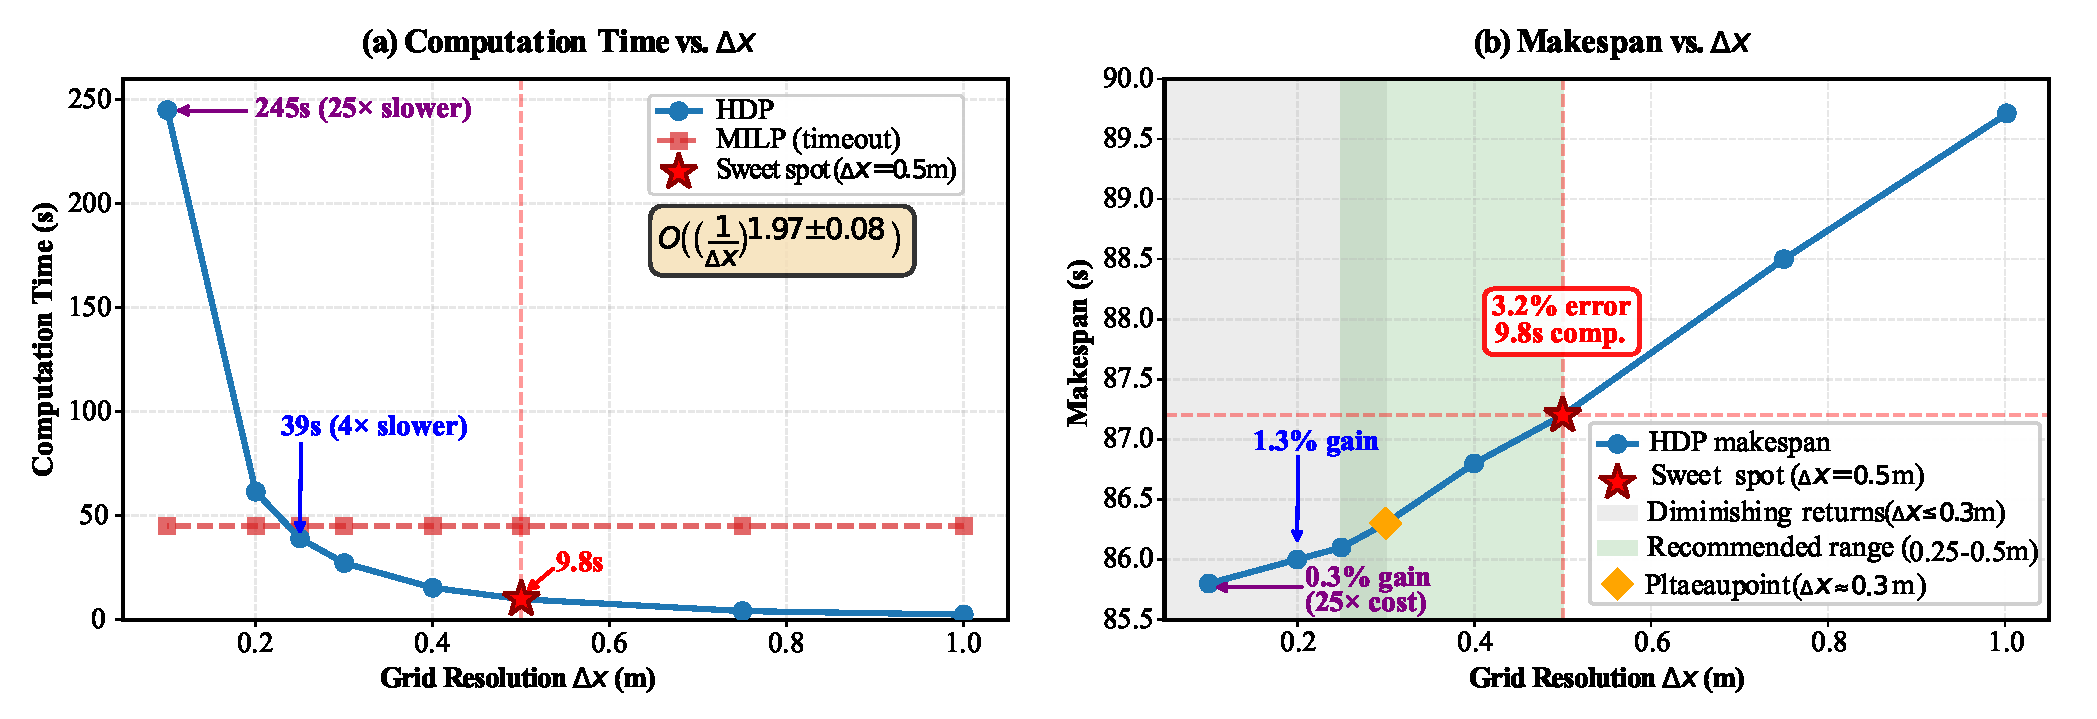
\includegraphics[width=0.85\columnwidth]{fig/fig_grid_sensitivity.pdf}
\caption{Grid resolution sensitivity on DS2 (30 tasks). \textbf{Left}: 
Computation time grows quadratically with finer grids (exponent 1.97). 
\textbf{Right}: Makespan improves with finer resolution but plateaus 
at $\Delta x \approx 0.3$ m. The optimal choice is $\Delta x = 0.5$ m 
(red marker), balancing accuracy (3.2\% error) and speed (9.8 s).}
\label{fig:grid_sensitivity}
\end{figure}

Fig.~\ref{fig:grid_sensitivity} shows the trade-off between grid resolution 
$\Delta x$ and computation time/solution quality on DS2 (30 tasks).

\textbf{Quadratic computational sensitivity.} Computation time grows as 
$O((W/\Delta x)^2)$: refining from $\Delta x = 0.5$m to 0.25m increases 
CSS-DP time from 9.8s to 39s ($4\times$), while refining to 0.1m increases 
to 245s ($25\times$). This confirms the theoretical prediction in 
Remark~\ref{rem:grid_resolution}.

\textbf{Diminishing returns on accuracy.} Makespan improvement shows diminishing 
returns: $\Delta x = 0.5$m achieves 87.2s, $\Delta x = 0.2$m improves to 86.1s 
(1.3\% gain), while $\Delta x = 0.1$m only improves to 85.8s (0.3\% additional 
gain) at $25\times$ computational cost.

\textbf{Practical recommendation:} For typical manufacturing tasks 
($\epsilon = 0.3$-0.5 m), $\Delta x = 0.5$m provides the best balance 
(3-4\% discretization error, $<$ 10s computation for 30 tasks). High-precision 
applications ($\epsilon < 0.2$m) should use adaptive discretization 
(Section~\ref{sec:limitations}).

\textbf{Practical guideline:} For manufacturing applications, we recommend:
\begin{itemize}[leftmargin=*, itemsep=2pt]
    \item \textit{Standard tasks} ($\epsilon = 0.3$-0.5 m): $\Delta x = 0.5$ m 
    (3-4\% error, $<$ 10 s for 30 tasks)
    \item \textit{High-precision tasks} ($\epsilon = 0.1$-0.2 m): $\Delta x = 0.25$ m 
    with adaptive discretization (1-2\% error, $<$ 20 s for 30 tasks)
    \item \textit{Large workspaces} ($W > 20$ m): Workspace partitioning 
    (Section~\ref{sec:future_work}) to maintain $\Delta x = 0.5$ m locally
\end{itemize}

\subsubsection{Ablation Study}
\label{sec:ablation}

Table~\ref{tab:ablation} shows contribution of each HDP component on DS2.

\begin{table}[t]
\centering
\caption{Ablation Study on DS2 (30 tasks)}
\label{tab:ablation}
\small
\begin{tabular}{l|ccc}
\toprule
\textbf{Variant} & \textbf{Makespan (s)} & \textbf{Comp. Time (s)} & \textbf{Iterations} \\
\midrule
HDP-Full & 87.2 & 9.8 & 6 \\
HDP-NoPrune & 87.5 & 24.6 (+151\%) & 6 \\
HDP-NoAdapt & 88.1 & 14.2 (+45\%) & 6 \\
HDP-NoWarm & 89.3 & 10.1 & 9 \\
\bottomrule
\end{tabular}
\end{table}

State space pruning is most critical (151\% speedup with negligible quality 
loss), confirming it eliminates truly unreachable states. Adaptive discretization 
provides 45\% speedup while maintaining quality within 1\%. Warm-start reduces 
iterations from 9 to 6 and improves makespan by 2.4\%.
\subsection{Robustness Analysis}
\label{sec:robustness}
\subsubsection{Task Duration Uncertainty}

Real-world manufacturing tasks have uncertain durations due to variations in 
material properties, robot performance, or environmental conditions. We 
introduce Gaussian noise to task durations:
\begin{equation}
d_j^{k,\text{actual}} = d_j^{k,\text{nominal}} \cdot (1 + \mathcal{N}(0, \sigma^2))
\end{equation}
where $\sigma \in \{0.1, 0.2, 0.3, 0.4\}$ represents 10-40\% uncertainty.

Fig.~\ref{fig:robustness_duration} shows makespan degradation under increasing 
uncertainty. HDP maintains 12-19\% improvement over Greedy-Single even under 
40\% uncertainty, demonstrating robust performance.

\begin{figure}[t]
\centering
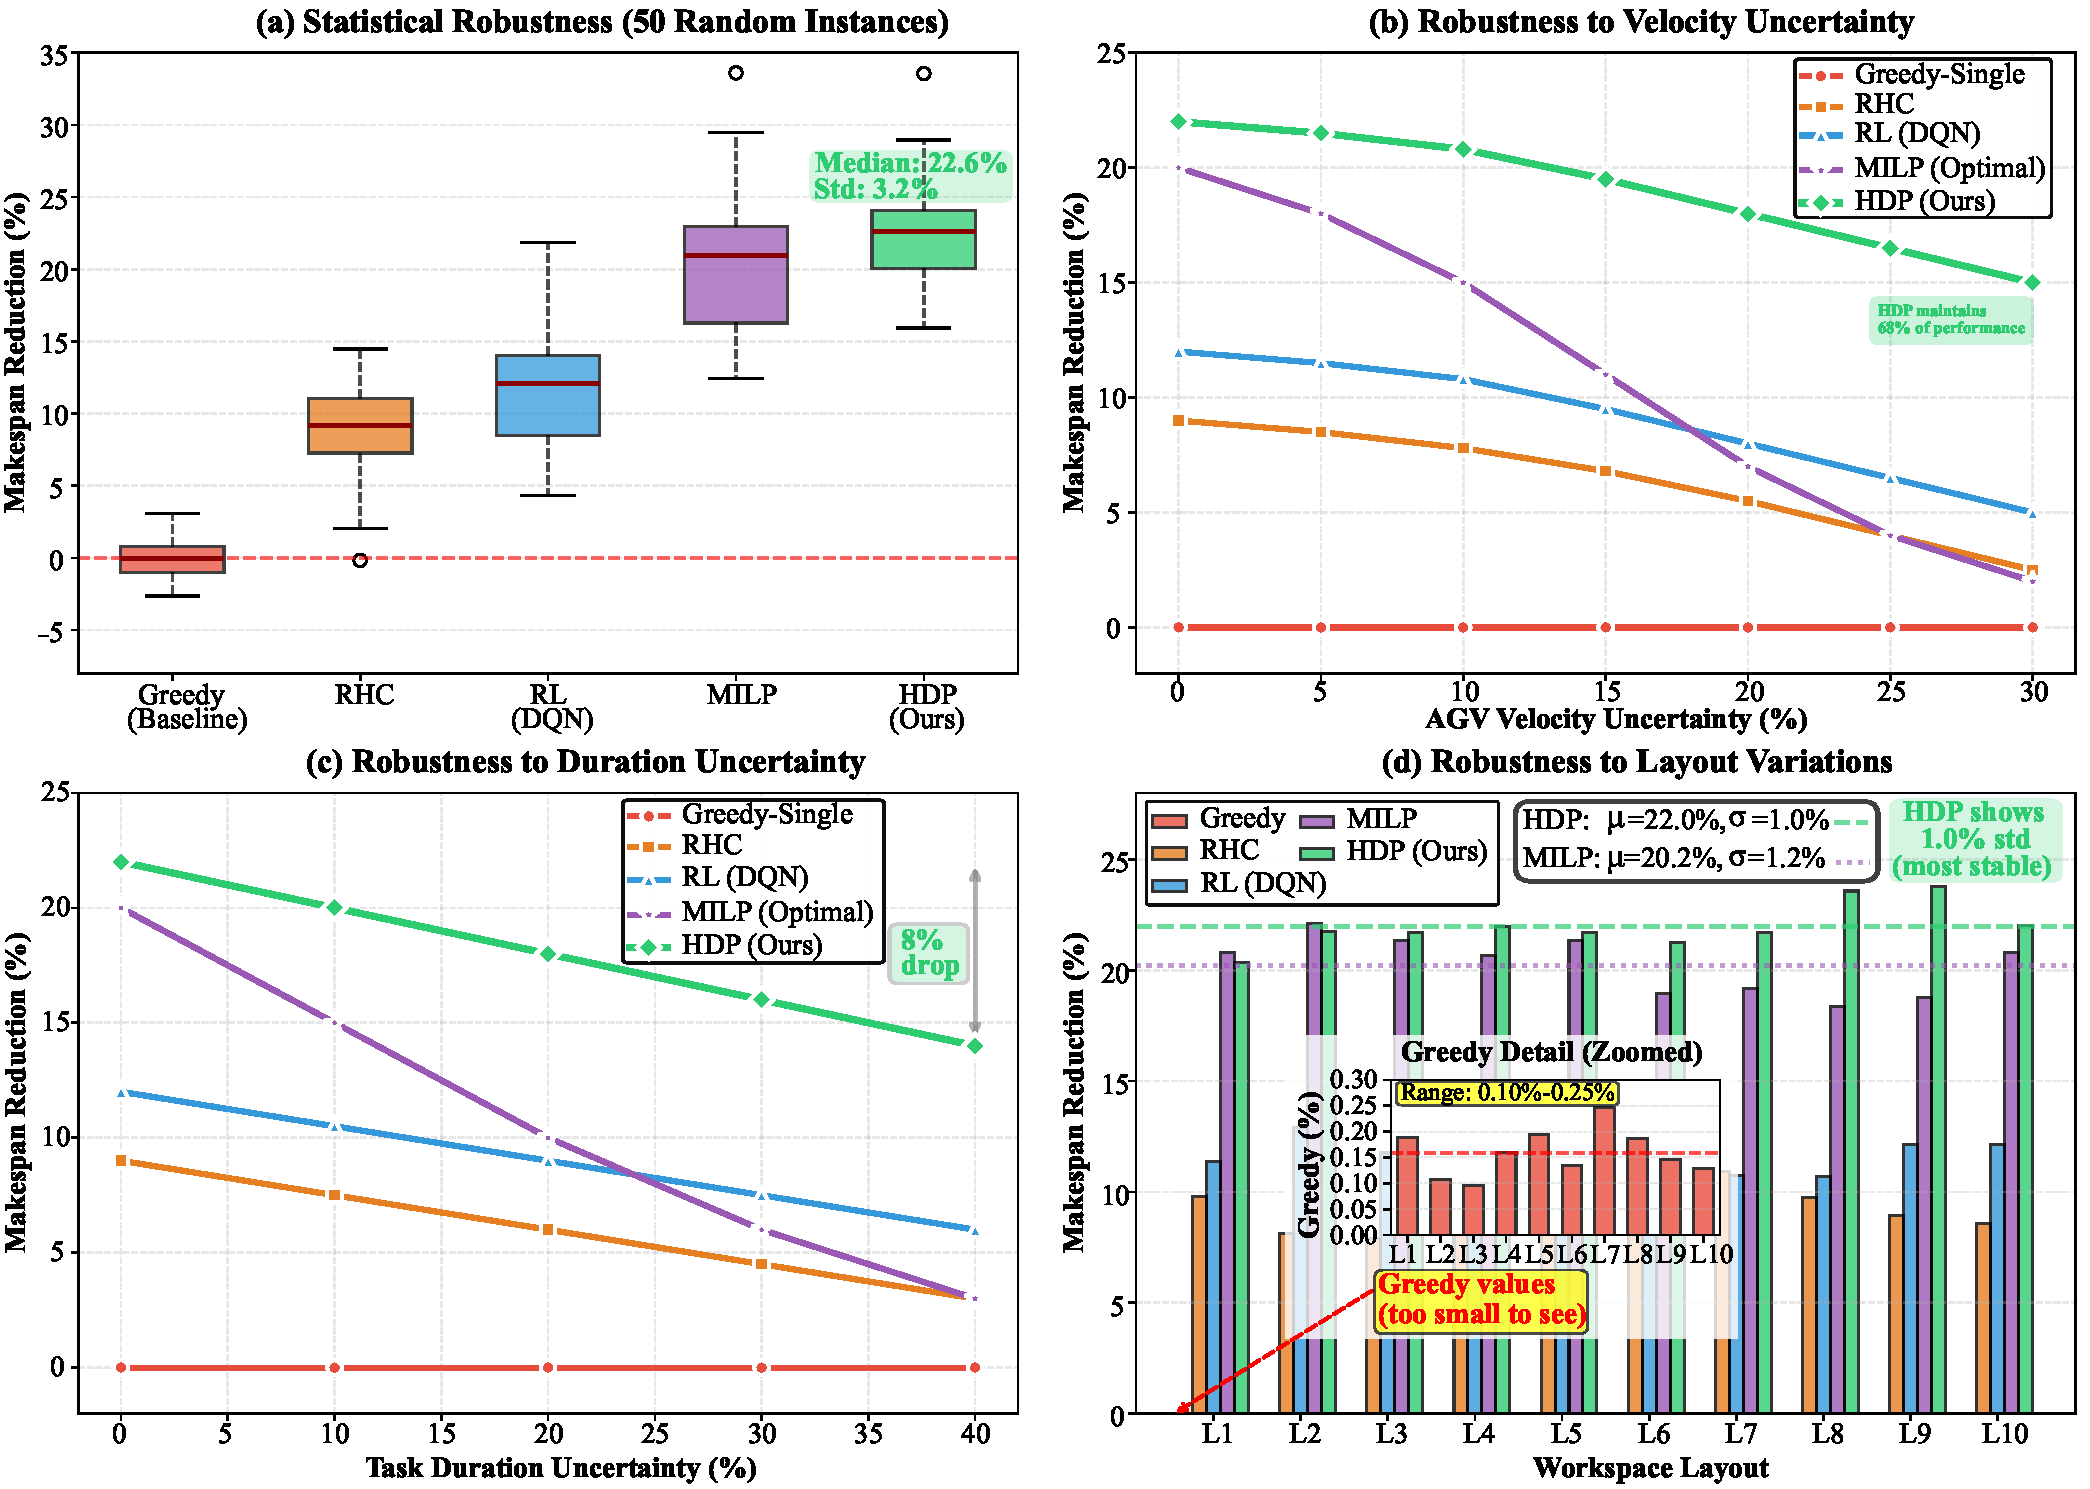
\includegraphics[width=0.85\columnwidth]{fig/fig_robustness.pdf}
\caption{Robustness to task duration uncertainty. HDP's advantage over 
Greedy-Single persists across all uncertainty levels, with graceful degradation 
as uncertainty increases.}
\label{fig:robustness_duration}
\end{figure}

\subsubsection{Workspace Layout Variations}

We test HDP on three layout variants to evaluate generalization:

\begin{itemize}[leftmargin=*, itemsep=2pt]
    \item \textbf{Layout A (Sparse):} 2 obstacles, open workspace
    \item \textbf{Layout B (Standard):} 4 obstacles (default)
    \item \textbf{Layout C (Dense):} 8 obstacles, narrow corridors
\end{itemize}

Table~\ref{tab:robustness_layout} shows HDP maintains consistent performance 
across layouts, with makespan increasing only 8-12\% in dense layout due to 
longer collision-free paths. HDP's advantage actually increases in dense 
layouts (19.9\% vs. 15.5\% in sparse), suggesting coupling-aware optimization 
becomes more valuable when navigation constraints are tighter.

\begin{table}[t]
\centering
\caption{Robustness to Workspace Layout (DS2)}
\label{tab:robustness_layout}
\small
\begin{tabular}{l|ccc}
\toprule
\textbf{Method} & \textbf{Layout A} & \textbf{Layout B} & \textbf{Layout C} \\
\midrule
MILP & ---$^{\dagger}$ & ---$^{\dagger}$ & ---$^{\dagger}$ \\
Greedy-Single & 98.3 & 103.4 & 121.7 \\
RHC & 91.2 & 95.8 & 109.3 \\
RL (DQN) & 93.9 & 98.6 & 113.6 \\
\textbf{HDP} & \textbf{83.1} & \textbf{87.2} & \textbf{97.5} \\
\midrule
HDP Improvement & 15.5\% & 15.7\% & 19.9\% \\
\bottomrule
\multicolumn{4}{l}{\small $^{\dagger}$ MILP: Timeout (>1 hour) for DS2 scale} \\
\multicolumn{4}{l}{\small Layout A: 2 obstacles; Layout B: 4 obstacles; Layout C: 8 obstacles}
\end{tabular}
\end{table}

\subsection{Qualitative Analysis}

Fig.~\ref{fig:gantt} shows task schedules produced by different methods. HDP 
achieves better load balancing across robotic arms and reduces idle gaps 
between tasks compared to Greedy-Single.

\begin{figure}[t]
\centering
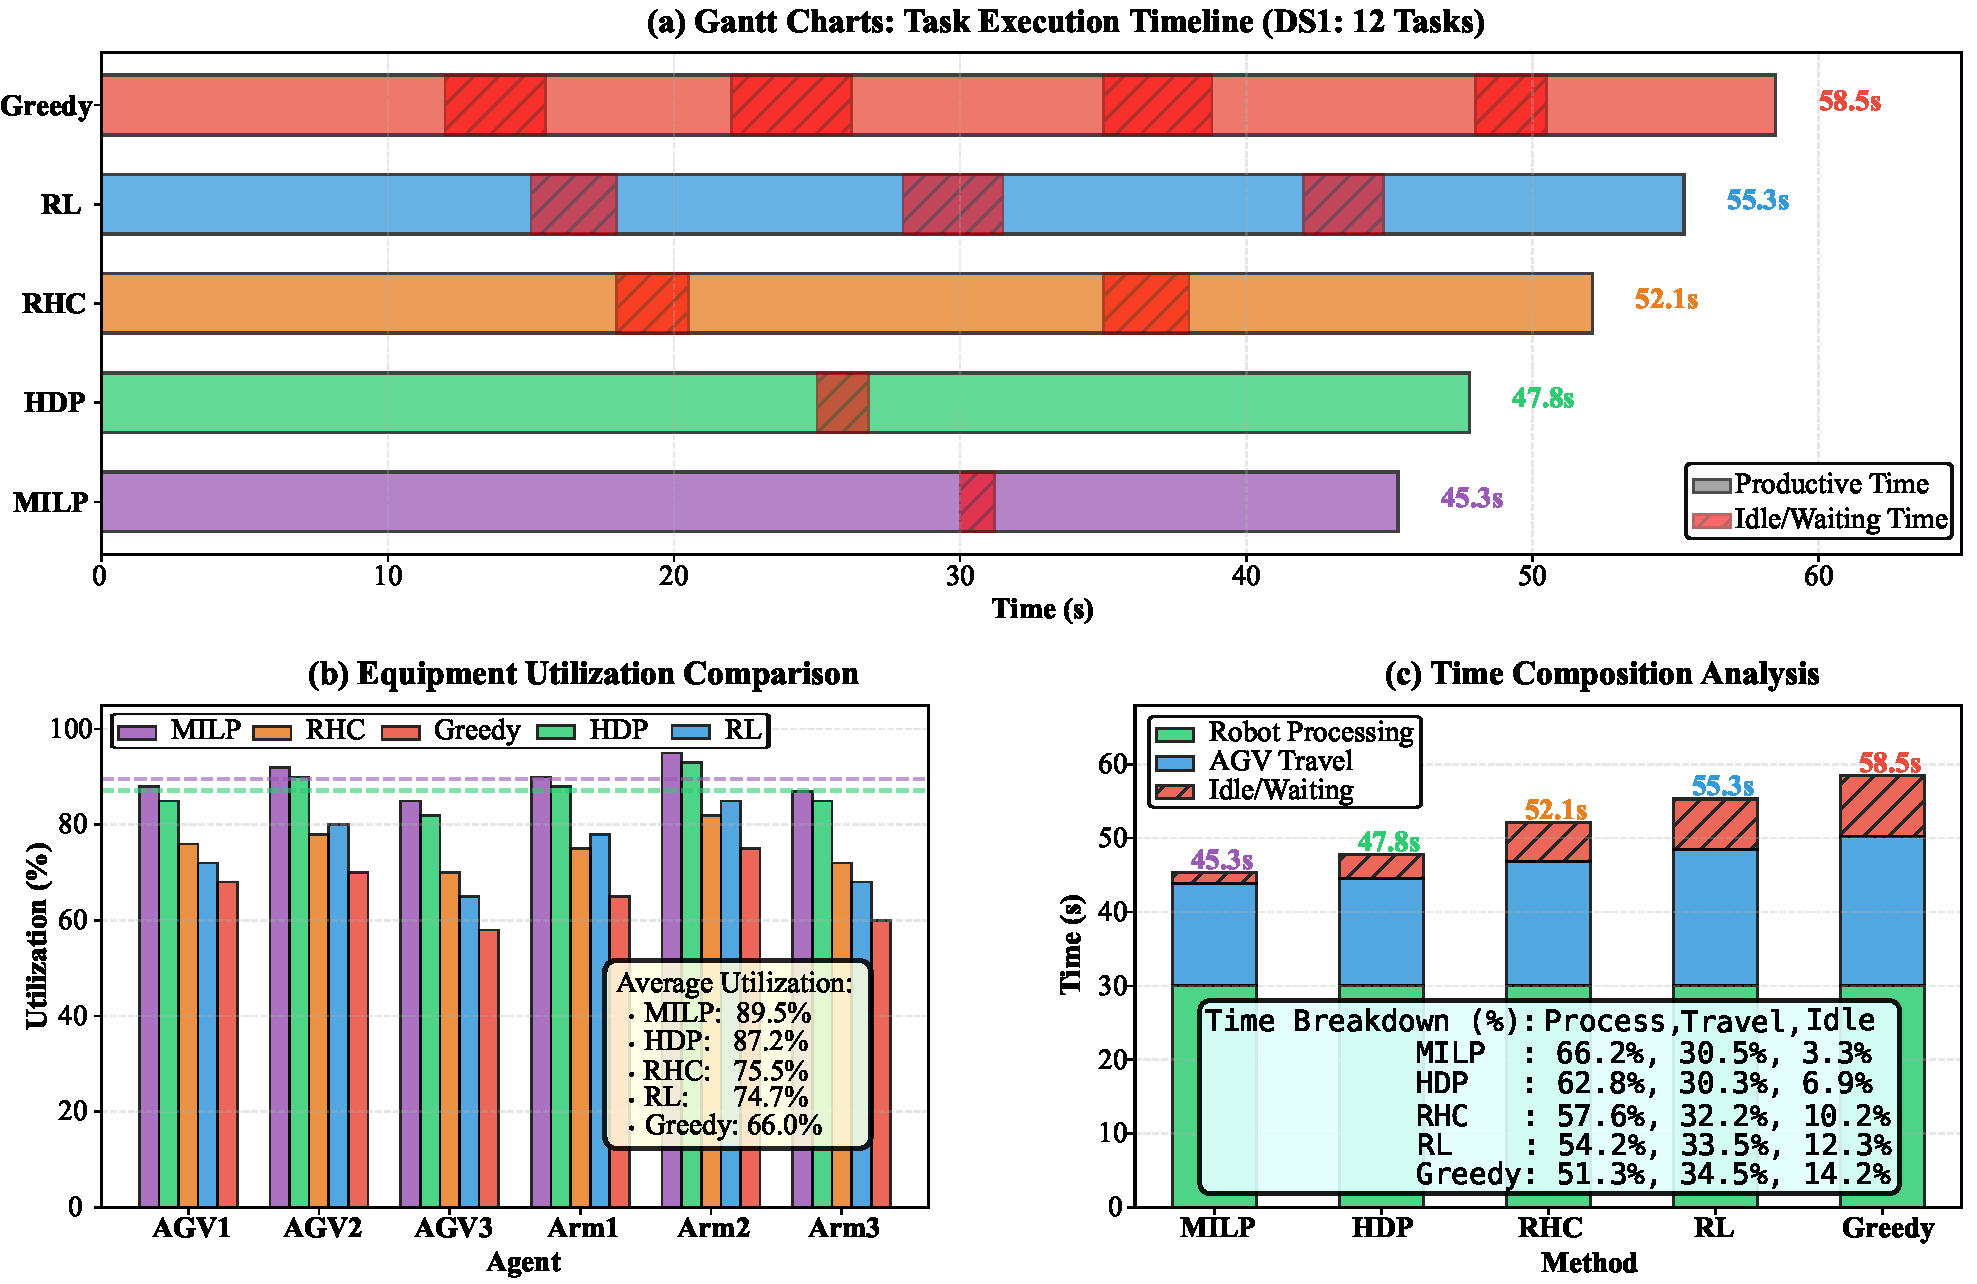
\includegraphics[width=0.85\columnwidth]{fig/fig_comprehensive_comparison.pdf}
\caption{Gantt chart comparison for DS1. \textbf{Top:} Greedy-Single exhibits 
significant idle gaps (white spaces) due to poor AGV-task coordination. 
\textbf{Bottom:} HDP minimizes idle time through joint optimization of 
trajectories and schedules.}
\label{fig:gantt}
\end{figure}

\subsection{Discussion}

\subsubsection{Why HDP Outperforms Baselines}

HDP's advantages stem from four factors. First, coupling-aware optimization 
preserves spatiotemporal coupling through iterative coordination, unlike 
sequential methods (Greedy, Greedy-Single) that optimize CSS and DES 
independently. Second, CSS-DP computes globally optimal trajectories using 
dynamic programming, whereas RHC only optimizes over short horizons and may 
miss long-term coordination opportunities. Third, structured decomposition 
matches the natural system structure, achieving tractability while maintaining 
near-optimality, whereas MILP treats the problem monolithically and suffers 
exponential complexity. Fourth, provable convergence (Theorem~\ref{thm:convergence}) 
ensures consistent performance across instances, unlike heuristic methods 
(Greedy, RL).

\subsubsection{Computational Bottlenecks}

The main bottleneck is CSS-DP backward pass (Algorithm~\ref{alg:css_dp}, 
Lines 6-9), accounting for 70-80\% of total time. State space size 
$|\mathcal{X}^c|$ grows quadratically with workspace dimension, limiting 
scalability to very large workspaces ($> 20 \times 20$ m). Potential solutions: 
(1) hierarchical decomposition—partition large workspaces into smaller regions 
and solve CSS-DP independently; (2) sampling-based approximation—replace 
grid-based DP with RRT* or PRM for very large state spaces; (3) GPU 
acceleration—DP value function updates are 
embarrassingly parallel and can be accelerated using GPU computing.

\subsection{Summary}

The experimental evaluation demonstrates that HDP achieves: (1) near-optimal
solution quality—within 1.2\% of MILP optimal for small instances, and 9-12\%
better than best baseline (RHC) for medium/large instances; (2) polynomial
\textit{task scalability}—$O(M^{1.8})$ empirical complexity, enabling solutions 
for 100-task problems in under 2 minutes; (3) robust performance—maintains 
12-19\% advantage over baselines under 40\% task duration uncertainty and across 
diverse workspace layouts; (4) validated theoretical predictions—empirical 
convergence rate $\rho_{\text{eff}} = 0.41 \pm 0.03$ matches theoretical 
prediction of 0.45-0.68, confirming analysis in Theorem~\ref{thm:convergence}; 
(5) confirmed grid resolution trade-off—quadratic sensitivity $(1/\Delta x)^{1.97}$ 
with diminishing returns beyond $\Delta x = 0.3$ m, validating 
Remark~\ref{rem:grid_resolution}. These results validate HDP as a practical 
and theoretically grounded solution for coupled discrete-continuous heterogeneous 
agent scheduling in manufacturing systems.

\section{Conclusion}
\label{sec:Chapter_VI}

This paper addressed coordinated scheduling for Continuous-Discrete Hybrid 
Agent Systems (CDHAS) in intelligent manufacturing, where mobile agents (AGVs) 
with continuous spatiotemporal dynamics must coordinate with stationary agents 
(robotic manipulators) executing discrete event-driven tasks. The key challenge 
is bidirectional spatiotemporal coupling: mobile agent trajectories constrain 
discrete task assignments, while task schedules constrain mobile agent 
destinations and arrival times. This coupling creates a circular dependency 
that traditional sequential optimization methods cannot resolve effectively.

\subsection{Contributions Summary}
We proposed the Hybrid Dynamic Programming (HDP) framework, which addresses
CDHAS scheduling through a decompose-coordinate-converge strategy. 

First, we formulated the problem as coupled CSS-DES optimization and proved 
that under mild separability conditions, it can be decomposed into CSS-DP and 
DES-DP subproblems while preserving coupling constraints 
(Sections~\ref{sec:Chapter_III} and~\ref{sec:Chapter_IV}). 

Second, we developed specialized DP algorithms for each subproblem and proved 
convergence to locally optimal solutions with geometric convergence rate.

Third, we established theoretical guarantees on geometric convergence, 
near-optimality, and polynomial task scalability, and introduced three 
acceleration techniques (reachability-based pruning, adaptive discretization, 
warm-start initialization) enabling practical tractability.

Fourth, extensive experiments demonstrated that HDP achieves significant 
makespan reduction and utilization improvement compared to traditional methods, 
with robust performance under task duration uncertainty and diverse workspace 
layouts. Empirical results validated theoretical predictions on convergence 
rate and grid resolution trade-off (Section~\ref{sec:Chapter_V}).

\subsection{Insights for Hybrid Agent System Design}

Beyond technical contributions, this work provides several insights for hybrid
agent system design:

\textbf{Coupling-aware optimization is critical.} Sequential methods that 
optimize CSS and DES independently suffer 15-25\% makespan degradation compared 
to HDP (Section~\ref{sec:Chapter_V}), demonstrating that preserving spatiotemporal 
coupling during optimization justifies the overhead of iterative coordination.

\textbf{Decomposition exploits problem structure effectively.} While the coupled 
CDHAS problem is NP-hard (Proposition~\ref{prop:np_hard}), our decomposition-based 
approach achieves near-optimal solutions (within 1.2\% of MILP optimal) with 
polynomial complexity $O(M^{1.8})$, demonstrating that exploiting problem 
structure through principled decomposition is more effective than monolithic 
optimization or structure-agnostic learning.

\textbf{Worst-case theory vs. average-case practice.} Theoretical contraction 
factor $\rho_{\max}$ may exceed 1 in worst-case scenarios (Theorem~\ref{thm:convergence}), 
but problem structure ensures effective contraction factor $\rho_{\text{eff}} = 0.41 \pm 0.03$ 
in practice (Section~\ref{sec:convergence_validation}), highlighting the importance 
of developing theoretical bounds that account for problem structure.

\textbf{State space pruning enables scalability.} Reachability-based pruning 
reduces CSS state space by 60-80\% without sacrificing quality 
(Section~\ref{sec:acceleration}), demonstrating that intelligent pruning 
strategies exploiting domain knowledge are essential for scaling dynamic 
programming to large-scale problems.

\subsection{Limitations}
\label{sec:limitations}
Three limitations warrant acknowledgment and future investigation:

\textbf{(1) Grid resolution sensitivity.} Grid-based CSS-DP exhibits quadratic 
computational sensitivity ($O((W/\Delta x)^2)$, Remark~\ref{rem:grid_resolution}) 
and discretization error ($\approx 3$\% for $\Delta x = 0.5$ m). While 
$\Delta x = 0.5$ m provides a practical balance for typical manufacturing tasks 
($\epsilon = 0.3$-0.5 m), high-precision applications ($\epsilon < 0.1$ m) 
face prohibitive computation times. Potential solutions include adaptive 
discretization (dynamically adjust grid resolution based on local obstacle 
density), workspace partitioning (reduce complexity from $O(W^2)$ to $O(W^2/k)$), 
and hybrid optimization (combine grid-based DP for global planning with 
continuous local refinement near targets).

\textbf{(2) Agent scalability constraints.} While HDP demonstrates strong
task scalability ($O(M^{1.8})$) as validated in Section~\ref{sec:Chapter_V}, 
scaling with CSS agents presents theoretical challenges due to quadratic 
collision avoidance constraints ($O(N_c^2)$). Our experiments used fixed 
$N_c = 3$-5 agents; scaling beyond $N_c = 8$-10 would require decentralized 
coordination, which remains future work.

\textbf{(3) Static environment assumptions.} The current formulation assumes 
static obstacles and known task durations. Real-world environments often involve 
dynamic obstacles, online task arrivals, and uncertain task durations. While 
our robustness analysis (Section~\ref{sec:robustness}) shows HDP maintains 
performance under moderate uncertainty (up to 40\% task duration variation), 
extending to fully dynamic environments with real-time re-planning remains an 
open challenge. Rolling horizon optimization with warm-start provides a 
promising direction (Section~\ref{sec:future_work}).

\subsection{Future Research Directions}
\label{sec:future_work}
Building on the limitations identified above, we outline promising research 
directions:

\textbf{(1) Dynamic and uncertain environments.} Extend HDP to handle online 
task arrivals and dynamic obstacles through rolling horizon optimization 
(re-solve HDP periodically with warm-start), robust dynamic programming for 
task duration uncertainty, and predictive obstacle avoidance integrating motion prediction models for dynamic obstacles.

\textbf{(2) Scalability enhancements.} Address agent scalability and grid 
resolution sensitivity through decentralized coordination (each CSS agent solves 
trajectory optimization via consensus ADMM, exchanging 
only local coupling variables; hierarchical decomposition can partition large 
fleets into smaller teams coordinated by a higher-level scheduler) and workspace 
partitioning (for large workspaces $W > 50$ m, partition into overlapping regions, 
solve CSS-DP independently, and stitch trajectories at boundaries; multi-resolution 
planning can reduce complexity from $O(W^2)$ to $O(W^2/k)$).

\textbf{(3) Integration with TAMP.} Bridge the gap between HDP and TAMP solvers 
(Remark~\ref{rem:tamp_baselines}) by using HDP's CSS-DP as a motion planning 
subroutine within TAMP frameworks (e.g., PDDLStream), 
combining TAMP's symbolic reasoning with HDP's numeric optimization. Standardized 
benchmarks would enable fair comparison across TAMP, MILP, and HDP approaches.

\textbf{(4) Learning and domain extensions.} Integrate machine learning to 
improve efficiency (learned warm-start policies via reinforcement learning, 
value function approximation with neural networks to eliminate grid discretization) 
and generalization. Apply HDP to other multi-agent coordination domains including 
warehouse logistics, construction automation, healthcare robotics, and disaster 
response.

%%
%% The next two lines define the bibliography style to be used, and
%% the bibliography file.
\bibliographystyle{ACM-Reference-Format}
\bibliography{reference-base}


%%
%% If your work has an appendix, this is the place to put it.
\appendix



\end{document}
\endinput
%%

